
While \cref{chap:alloy} explore ways to identify topical-based options for scenarios that involves deep understanding of a handful of different solutions, such as gardening, pluming, and physics, this chapter explore a different set of exploratory search scenarios where there are a much larger number of entity-based options available. For example, planning a trip or shopping for products where it can involve intense cross referencing of multiple sources for a large set of entity options. One has to determine the popularity and trustworthiness of competing options and avoid missing valuable but less common options. Traditional search systems leave this task to users, while automatic result clustering approaches often fail to produce structures coherent enough to meet these needs. We introduce a novel approach that builds coherent topical landscapes from search results. By combining the rich but sparse representations of knowledge bases with word vector models that are shallow but dense in coverage, we produce structures more coherent than alternative approaches. We instantiate this in a prototype interactive system and explore which elements users find useful. Across three information seeking scenarios, we found that participants valued both the structure and distribution information provided by our system for complex exploratory searches and, surprisingly, simple searches as well.  
%    Whether planning a trip or researching medical symptoms, many complex exploratory search tasks involve scenarios where users are unfamiliar with the domain of interest, unsure about what the possible options are, and have difficulty knowing how popular or trustworthy those options may be.  Current approaches to supporting search either fail to address these needs or are limited by a dependence on the existence of well-structured metadata. We introduce a novel approach to extracting structure from arbitrary web content (e.g., in a set of search result pages) and explore the value such content can provide in helping users understand the information landscape. The intuition behind the approach is that knowledge graphs and ontologies provide rich but sparse representations that can be used to structure search landscapes, while word vector models are shallow but work on a wide variety of terms and entities. We combine these methods to build interactive search landscapes that automatically discover relevant topics for a given query based on the content of the web pages and external knowledge sources, measure the distribution of topics across sources, and group topics into useful schemas. Across three information seeking scenarios we found that participants found our approach useful and an improvement to traditional search interfaces for complex exploratory searches and, surprisingly, simple searches as well.



%From simple fact-finding tasks to complex learning and information exploration tasks, people often rely foraging information online to make sense of the world today. Particularly, exploratory searches that involves learning in an unfamiliar domain can often be stressful and time consuming. While modern search engines do a great job at retrieving intended webpages in split seconds, searchers in these scenarios often do not have clear ideas about the exact information needed \cite{mar2006exp}.
%In contrast to previous work that focused on shepherding users to intended documents using structures in labeled corpora, we focused on 
%combining hand-crafted knowledge bases with machine learned semantic models to extract interpretable structures with good coverage
%from unstructured web content.
%This allowed us to surface the distribution of key subtopics, providing an overview of the information landscape. We embody this idea in an interface we called SearchScape, which allows searchers to gain quick overviews using the distribution of key subtopics, and interact with search results to dive into different subtopics. In an experiment with 210 participants and a 3x2 between subjects design, we tested SearchScape in a wide range of scenarios, and the effects of showing distribution information.
%Results showed that participants found SearchScape to be useful and an improvement to traditional search results interfaces, and that showing distribution of key subtopics was perceived as significantly more useful.



\begin{figure}
    \centering
    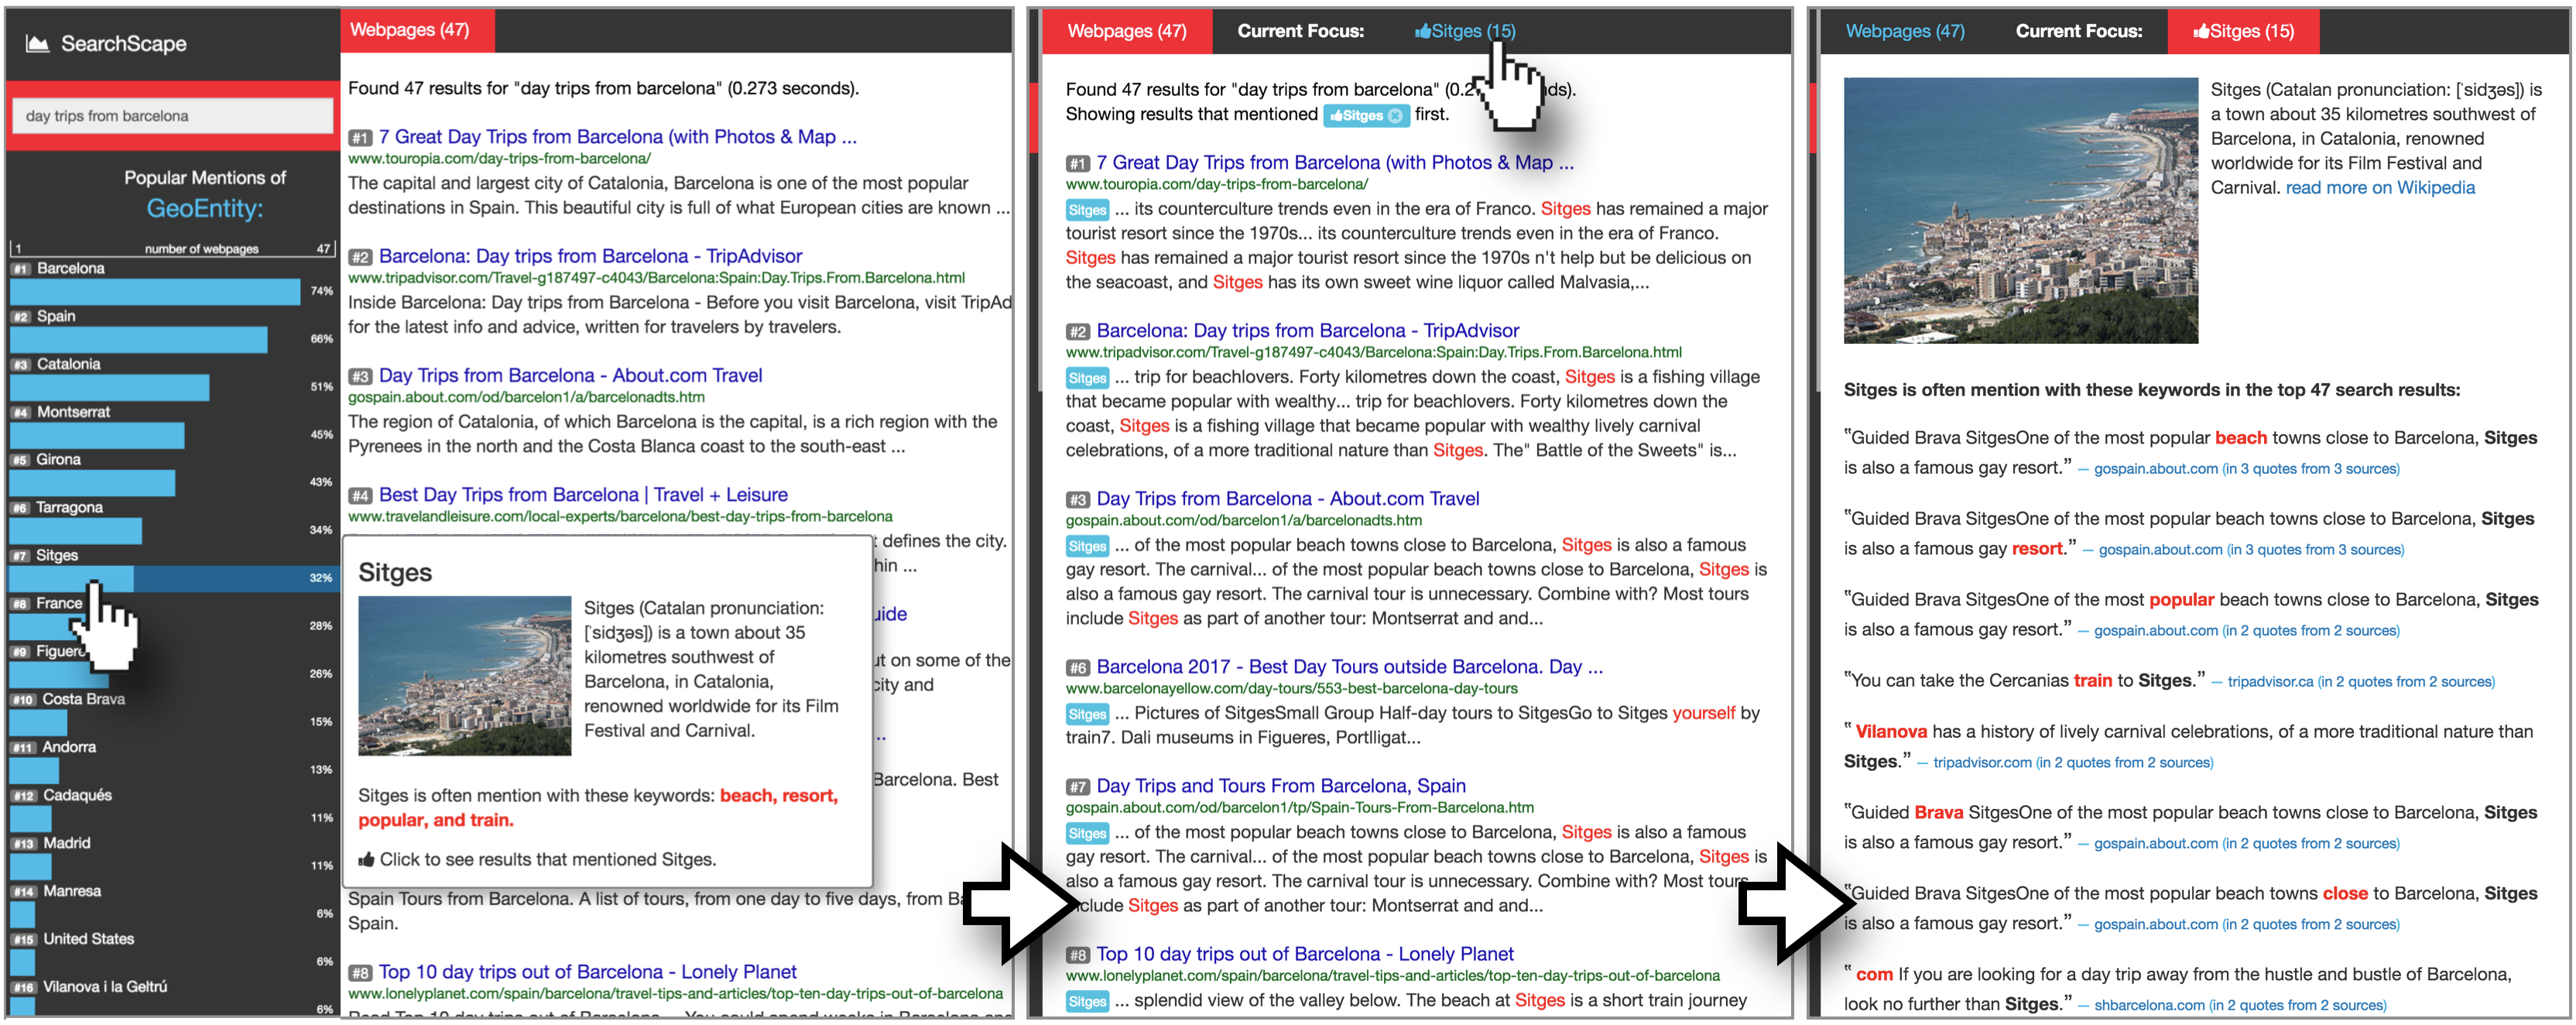
\includegraphics[width=1.0\textwidth]{Chapters/SearchScape/figures/main_old.png}
    \caption[An overview of the SearchScape system.]{An overview of the SearchScape system. The Document Panel on the right shows a ranked list of search results, while the Structure Panel on the left shows the distribution of automatically identified key concepts in the search results. Exploratory searchers can click on an item to filter the search results and see how the item of interest is mentioned across sources. Alternatively, they can also grouped these mentions using keywords were frequently mentioned together with the item of interest.}
    \label{fig:flow}
\end{figure}

\section{Introduction}

Consider an example of an exploratory search such as looking for the best day trips from Barcelona. Searching for this online returns a set of web pages primarily composed of lists of day trip destinations. These range from the popular beach town of Sitges to the less well known market town of Vic. However, looking at any single page raises a number of potential issues. A reader might want to know the relative popularity of each option: while Sitges appears many different sources, Vic appears in only a few, despite being given approximately equal weight on a top search result.\footnote{LonelyPlanet - Top 10 day trips out of Barcelona,  https://www.lonelyplanet.com/spain/barcelona/travel-tips-and-articles/top-ten-day-trips-out-of-barcelona} Conversely, a page may be missing a popularly cited option such as Sitges and the reader would have no indication they might be missing out.  Providing an overview of the range of options could also expose interesting options in the long tail that could be relevant to certain readers, despite not appearing in the top few results (e.g., a Utopian textile mill's church designed by Gaudi, Col\`onia G\"uell).  

To understand the prevalence of this problem, we conducted a pilot survey with 103 participants from Amazon Mechanical Turk (age between 20 and 63, M=36, SD=12, 60\% male and 40\% female, mostly from the US), focusing on their experiences when conducting complex exploratory searches. Around half of the participants reported having conducted more than four exploratory search tasks in the past two weeks, in which 17\% reported having conducted more than ten tasks. Our results reaffirm that 
when conducting exploratory searches, people read from multiple information sources to make sure they do not miss something important (84\%), look for more information about a topic from other webpages in the same search result (84\%), verify previously seen but uncertain information using multiple sources (88\%),
and get a sense of what's popular or important in the search results (76\%).
At the same time, many also found conducting complex searches can be stressful (60\%), and that they often end up with more browser tabs than they can manage efficiently (67\%). These findings are consistent with previous findings that shows that up to 33\% of this time is related to complex exploratory search tasks \cite{mar2006exp,kellar2007field,rose2004understanding}.



%To address these challenges searchers actively engage activities such as cross-referencing information across different webpages, identifying and learning important subtopics, planning out subsequent queries (cite), and synthesizing information gathered from multiple sources (cite something from KA).


Despite their importance and ubiquity, the activities described above are poorly supported by modern approaches. Recent advances in search interfaces have optimized for providing information as quickly as possible, such as knowledge cards in which an answer is surface directly on a search results page or visual carousels of possible options that a user can quickly click through. These approaches excel at finding specific information, but notably fail to address the activities involved in complex search such as cross-referencing information across different webpages, identifying and learning important subtopics, planning out subsequent queries, and synthesizing information gathered from multiple sources.

Meanwhile, research on supporting complex information seeking has attempted to address some of these activities through faceted navigation \cite{hearst2006design} and semantic web interfaces \cite{wilson2006mspace}. While useful in an environment with well-structured data, it's prohibitive to expand these approaches to support the unstructured Web \cite{bruce1999workplace,teevan2008challenges}.
%The most obvious challenge here involves the difficulty for computational approaches to automatically detect important subtopics and information items from the general and unstructured search results }. 
One promising direction has been using unsupervised clustering algorithms to automatically extract structures from search results, which have been found useful for separating relevant sources from irrelevant sources (e.g., differentiating fruit related from technology related results when querying ``apple'') \cite{zeng2004learning}. However, these automatically generated structures are rarely coherent enough to provide an overview of the space of useful information. Consider the top five clusters that Clusty (now yippy.com) shows for ``Day trips from Barcelona'': Spain, Europe, Cruise, Photos, Reviews. Even within the Spain cluster the subclusters provide no structure or coherence: Blog, Tours from Barcelona, Flights, Guided, Cordoba, Cultural, etc.  The topics for ``Guacamole recipes'' similarly do not provide any concepts of the same class: Mexican (country), Chef (profession), Health (topic), Blog (format), and Free (cost). While these structures may be useful for navigating to sources in different dimensions (e.g., websites for guided tour services, for photo albums, or for blog posts), they provide little utilities for comparing between options under the same dimensions. For example, comparing the popularity and the types of activities you can do in different locations when searching for day trip destinations, or compare the reviews and popularity of different guided tour services. Fundamentally, automatic structures often provide no structure to define a space -- there is no base for comparison and no understanding of relationships between concepts in their structure. 
At a higher level, faceted search and clustering approaches make better filers for people to zero in on what they know they are searching for (e.g., Apple the tech company), whereas we are instead trying to provide an atlas for exploratory scenarios (e.g., how popular are the different destinations, and how different sources describe them): a representative description of the space to help searchers learn about their options in the information space and how key concepts are distributed among the search results.

%However, a more subtle issue is that even when metadata exists to support computational approaches, the way this information is exposed (e.g., through facets or clusters) is often oriented towards directing people to specific pages rather than providing them with an understanding of the distribution of information in the query space in a way that more directly supports the examples above. 

%A third possibility is that adding this extra information may complicate the search interface in a way that is undesirable for searchers, providing insufficient value for the added complexity.

In this chapter we explore a novel approach for extracting coherent structures from arbitrary unstructured web content (i.e., in a set of web search results), and also how to present such structures to the users to provide an overview of the information landscape. We instantiate this approach in a prototype system called SearchScape, an interactive search result exploration interface. SearchScape dynamically identifies useful structures by combining external knowledge bases (i.e., Wikipedia\cite{bollacker2008freebase} and NELL\cite{carlson2010toward}), and machine learned unsupervised semantic models (i.e., Word2Vec\cite{mikolov2013efficient} and GloVe\cite{pennington2014glove}). The intuition behind this approach is that on the one hand, knowledge bases provide high quality entities and ontological frameworks, but often lack good coverage over arbitrary search results. On the other hand, unsupervised models provide substantial coverage, but can often be overly generalized and difficult to understand due to its lack of structure and incoherence. SearchScape combines the two to identify high quality categories from  knowledge bases that are easy to understand (e.g., Geographic Locations, or Agricultural Products), while expanding the coverage of these categories using automatically learned semantic models. In our first study, we find that structures produced by SearchScape for 50 different exploratory search queries was found to be significantly more coherent than structures produced by a search result clustering system.

Extracting coherent structure enabled us to further expose the distribution of key items of the same classes in the search results, in hopes that it can allow exploratory searchers to better understand all the options in the information landscape. For example, exposing the popularity of different \emph{location} items when searching for day trip destinations, or how common different \emph{ingredient} items are when searching for recipes.  In our second study, the overall system was found to be useful for three diverse scenarios including both exploratory and fact finding search. Further examination using a control condition hiding distribution information found that in exploratory situations showing distribution was significantly more beneficial to searchers.





\section{Related Work}


Several exploratory search interfaces have been developed in order to help searchers orient themselves in the information space, review and explore the different subtopics, and keep track of their overall progress \cite{hearst2009search,marchionini2000agileviews,patterson2001predicting,tretter2013searchpanel,morris2008searchbar}. Two closely related studies include Topic-Relevance Map and Exploration Wall, which explored ways to provide overviews of search results of academic papers using document keywords and entities and easily choose keywords to build up subsequent queries \cite{peltonen2017topic,klouche2015designing}. SearchScape also makes use of key entity mentions in the document for overview and drill-down purposes, but we automatically extract key items from the unstructured web using combined hand-crafted knowledge bases and machine learned unsupervised semantic models.

%In SearchScape, we retain the look and feel of standard web search engine, but included an extra side panel to provide a quick overview of the information space, and also to enable deep interactions with the search results. 




\subsection{Diversity and Distribution of Information}

%Ensuring that the users are exposed to a diverse set of  information is crucial for discovery-oriented exploratory search tasks, but researchers have also found that queries formulated for the same exploratory search tasks often yielded highly overlapping sources up to 50\% to 60\% \cite{qvarfordt2013looking}. Consequently, a collection of research has focused on helping exploratory searchers reach more diverse results without drastically changing the existing search paradigms and interfaces. For example, providing real-time feedback during query formulation by suggestion different subtopics (cite auto complete for exploratory), or providing real-time visual previews of the proportion of overlapping sources during query formulation \cite{qvarfordt2013looking}. Researchers have also focused on the ranking and re-ranking to increase the diversity of search results. 

Initially motivated to reduce redundant information in top search results produced by traditional relevance-oriented ranking algorithms, Carbonell et. al first introduced the idea of ranking search results to increase the diversity of information in the top results for scenarios where a large amount of potential relevant document exists in the corpus \cite{carbonell1998use}. More recent research has also explored how diversifying search results can benefit exploratory searchers (e.g., \cite{jin2013interactive}). Our perspective differs from these pure diversity-oriented ranking approaches, which optimize for showing as many different topics to the user as possible. We instead argue that the distribution of different topics and key entities can actually be a useful signal for exploratory searchers to judge the importance of different subtopics, and prioritizing their subsequent exploration. In this case, showing a uniformly diversified list of search results could actually give people an incorrect sense of the information distribution. For example, showing as many restaurant choices as possible can at the same time obscure a sense of how frequently each restaurant is mentioned. A similar idea was pointed out by Dang et. al, who proposed instead to diversify search results while accounting for the proportionality of information in the search result \cite{dang2012diversity}. In SearchScape we take a more direct approach than re-ranking search results and  present the distribution of extracted entities on the interface so that exploratory searchers can easily compare and evaluate the different subtopics in the information space.

%Jin et. al proposed to diversify the top search results in the first page so that users can get an overview of the information space, and re-rank the rest of the results based on which webpages the users visits \cite{jin2013interactive}. 

%Researchers in the fields of cognitive psychology, human-computer interaction, and information retrieval have made great strides on both understanding the process of exploratory searches and building systems and interfaces to better support exploratory search scenarios (bunch of cites).  

%SearchScape differs from traditionally faceted search systems in two ways: 1) We automatically inferring categories and entities using external knowledge sources, instead of relying on labeled corpora. 2) Traditionally facets were primarily used for navigation and finding items that meet specific criteria. We instead use ``facets'' primarily to give users a sense of the information space, to expose information distribution, to show different contexts of use, and generally for exploration.



%However, these faceted exploratory search systems all exploited corpora that were manually labeled with carefully designed categories and facets, such as authors and publish dates of books, genres and lengths of movies, or brands and prices of merchandises. Much of the techniques cannot be easily utilized for the general web due to both the unreliability of online information sources, and the lack of readily available metadata for online documents beyond titles and domain names. Past efforts on using crowdsourced editors to categorize websites, such as the Open Directory Project\footnote{DMOZ, https://www.dmoz.org/}, had also failed to keep up with the ever scaling of the web, and most have been discontinued. In addition, online documents often describe multiple items on the same page (e.g., \emph{top 10 compact cameras}), which can make it difficult to uniquely categorize a document under a single category (e.g., a facet of camera brands). Secondly, many past systems used high quality corpora that were assumed to be trusted by their users. For example, the the price and brand information of products on commerce websites, or the author and publish date information on publisher websites, when conducting complex exploratory search for unfamiliar domains on the Internet, most searchers are actively evaluating the trustworthiness of information sources they have encountered using different types of features, such as domain names, visual designs, and writing styles(?) (cite web/trust papers), and often validate and evaluate the importance of a new piece of information by cross-referencing multiple sources (cite??? Maybe something in KA?). For example, choosing a travel destination that were frequently mentioned favorably online, or paying attention to the frequently discussed term ``recurrent neural-networks'' when researching ``artificial intelligent'' online. This lack of support in modern search interfaces for discovery-oriented exploratory search scenarios has left users the heavy burden of figuring out the important subtopics in the space of information using just a linear ranked list of relevant webpages \cite{bruce1999workplace}, leading them to rely on external tools such as printing, and word processors to deal with the issues of organizing, managing and re-finding previously found information \cite{aula2005information,white2006supporting,morris2008survey,capra2010tools,kittur2013costs}. 

\subsection{Faceted Search for Structured Corpus}

Faceted search is perhaps the most commonly used search interface, in which users can filter results by selecting or deselecting categories or ``facets'' (e.g., products on an online shopping site). Although originally designed to help searchers efficiently narrow down on relevant sources and exclude irrelevant sources from their search results (e.g., showing only digital cameras of specific price range and manufactured by a specific company on an online shopping site), researchers have also found faceted search interfaces to benefit exploratory scenarios, where searchers are less certain about their information needs \cite{hearst2002finding,yee2003faceted}. Facets can provide an  overview of the different topics in the information space in addition to supporting drill-down on those topics \cite{yee2003faceted,capra2008relation,kules2009exploratory} and have been widely explored for corpora where metadata are readily available, such as images \cite{yee2003faceted}, music \cite{wilson2006mspace}, social media \cite{o2010tweetmotif}, library catalogs \cite{marchionini2006towards,kules2009exploratory}, and scholarly articles \cite{hearst2009nlp,dork2012pivotpaths,klouche2015designing}. However, in cases where metadata is not readily available, computationally inferring fine-grained facets (e.g., day trip destinations) remains a challenge, inhibiting the faceted interface from being expanded to support exploratory search on the open Web \cite{bruce1999workplace,teevan2008challenges}. Instead of requiring documents to be annotated with metadata, SearchScape uses a novel technique for automatically producing structures by inferring topics from unstructured web content by combining readily available knowledge bases and ontologies. Furthermore, we also explore the benefits of visually depicting the distribution of content across structures in helping the user better understand the information space.


\subsection{Automatically Identifying Structure}

More generally, numerous challenges have been identified \cite{teevan2008challenges} in developing structured search systems to better support exploratory scenarios without pre-compiled metadata. Researchers have long explored ways to extract structure by clustering search results using machine learning \cite{zamir1999grouper,zeng2004learning,hearst1996reexamining}, lexical and HTML patterns \cite{kong2014extending}, crowdsourcing \cite{ka,alloy,cascade}, or interaction techniques \cite{hearst1996reexamining,hearst1996visualizing,hearst1996visualizing}. However, a number of papers \cite{hearst2006clustering,chuang2012interpretation,alloy} point to the fact that automatically techniques, such as unsupervised clustering, can often produce incoherent structures that are difficult to comprehend by users unfamiliar with the domain of interest. Further, providing a quick overview using coherent structures can be critical in supporting early stages of the exploratory search process. This helps users get a sense of the information space, and further investigate subtopics that are interesting or important to the them \cite{mar2006exp}. Conversely, techniques that utilize human judgments via crowdsourcing or user interaction can produce structures that are more coherent, but do so at the expense of either additional time and monetary cost or user effort\cite{alloy,ka}.

Perhaps most closely related to our work in intent, MetaSpider extracts noun phrases from webpages to use as features for clustering webpages in search results into visualized topic maps using the Kohonen SOM algorithm \cite{chen2001metaspider,kohonen1998self}.
Instead of trying to identify structures solely based on information presented in the search results, SearchScape utilizes rich and readily available knowledge bases and ontologies to automatically identify dynamic but coherent structures that best fit the search results.
%First, SearchScape identifies topics relevant to the current search results from large sets of predefined concepts in knowledge bases using their ontological frameworks, and then extracts entities of those topics from the search results to generate coherent and interpretable structures.
In addition, instead of producing document clusters, SearchScape presents distributions of entities over documents in the search results, as an overview of the information space (e.g., list of day trip destinations and how often they are mentioned in the search results.)

%For example, the Scatter/Gather system allowed users to navigate and explore large collections of documents using an interactive hierarchical clustering paradigm \cite{hearst1996reexamining}. The TileBars system allowed users to define topic models using sets of keywords, and provide real-time visual feedback for exploring the topic distributions over documents in search results \cite{hearst1996visualizing}. On the other hand,  







\section{System Design}
The SearchScape system augments standard web search results with a list of dynamically identified concepts useful for the current query. This gives exploratory searchers the ability to first gain a quick overview of the information space and explore different subtopics. The system consists of two main components. First, SearchScape analyzes the content of all webpages in the search results to identify the latent structures in the information space leveraging existing knowledge base structures (which typically have higher accuracy but lower coverage) and expands them with unsupervised word vector models (lower accuracy but higher coverage). Then, the search results along with the identified structures are presented to the user through an interactive search result interface which visually presents the distribution of structures. In the following subsections, we will describe in detail our data sources, the back-end components, and the front-end interface.

\subsection{Data Source}

In an ideal setting, the back-end components of SearchScape would be integrated as a part of a general web search engine, so that content fetching, indexing, and analysis can be performed before query time. However, since it would require enormous time and resources to download and index the entire web to build a full-scale web search engine, we used a readily available API from a commercial search engine as our data source.\footnote{Bing Web Search API, https://www.microsoft.com/cognitive-services/en-us/bing-web-search-api} In the front-end, SearchScape focused on augmenting traditional web search results with automatically identified, task-specific structures using an interactive interface to better support exploratory scenarios. Similar to search engine back-ends, we also pre-fetch and pre-index webpages for a fixed set of queries by first retrieving a list of top 50 relevant webpages from the API, then download and extract the main content of each webpage to remove menus and advertisements using an readily available API\footnote{Mercury Web Parser, https://mercury.postlight.com/} and build an inverted-index file for each webpages \cite{baeza1999modern}.
Finally, we perform further analysis to identify task-specific structures as described in the next subsection.\footnote{Many academia alternatives also exist for webpage content extraction such as \cite{kohlschutter2010boilerplate}.}

\subsection{Identifying Structures}

\begin{figure}
    \centering
    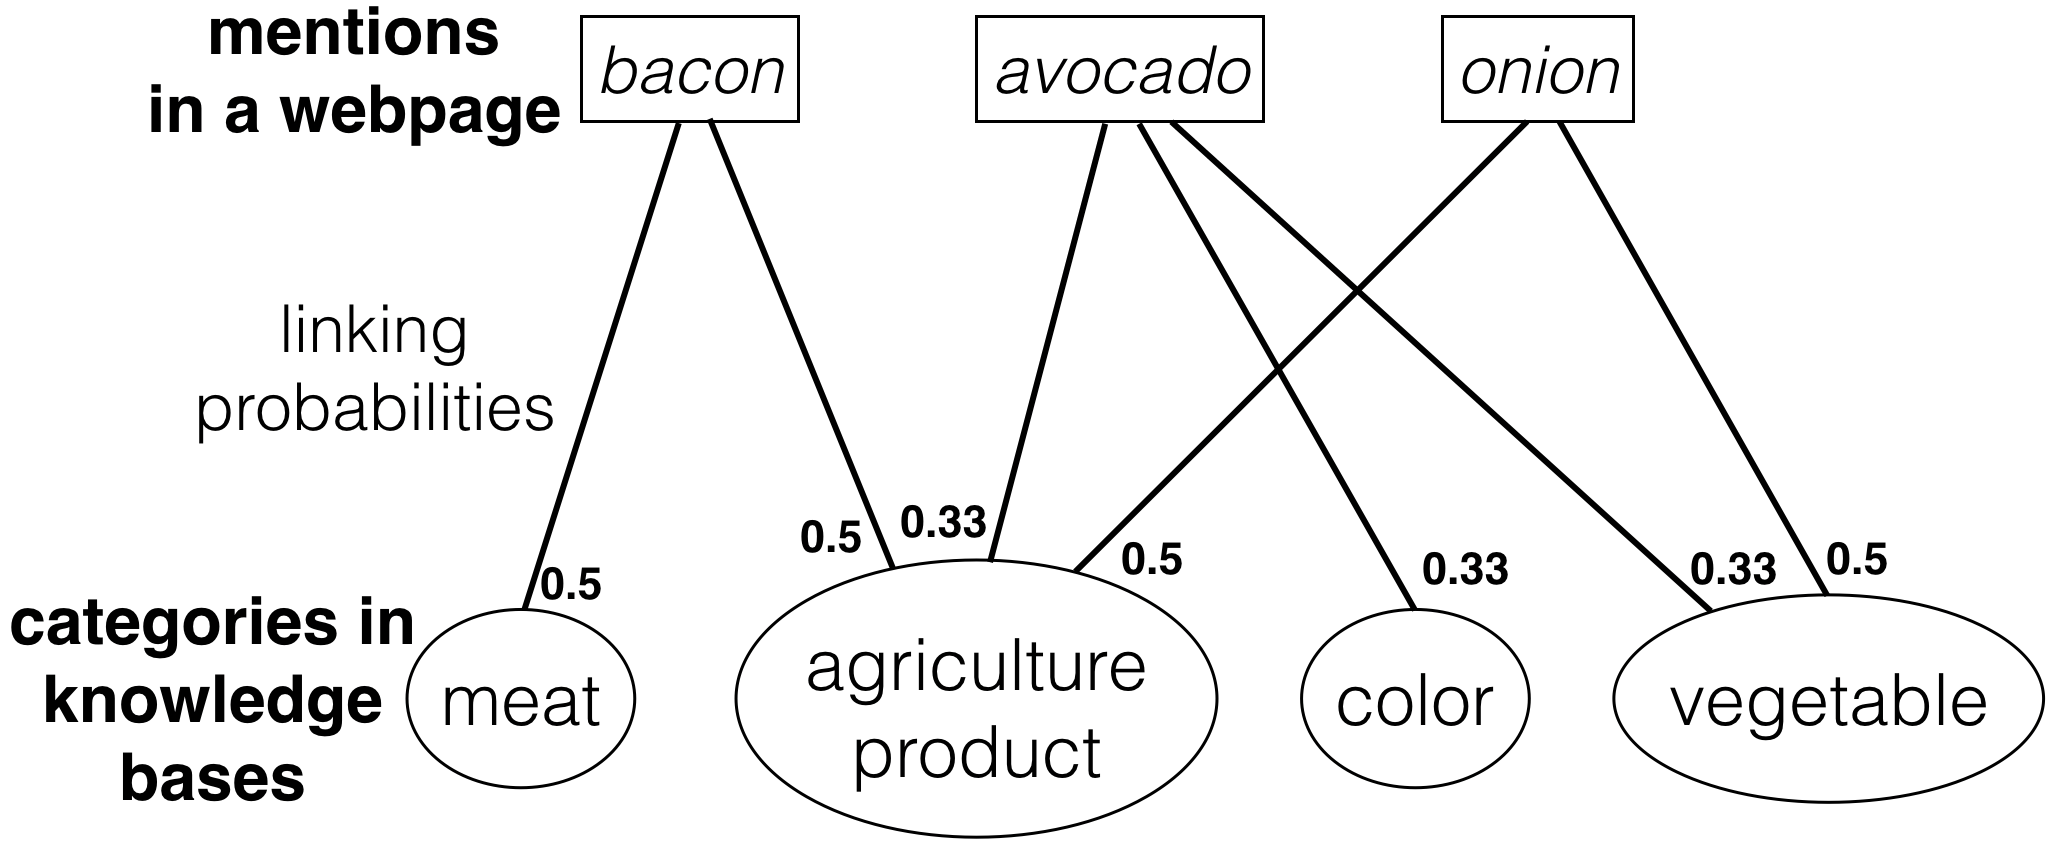
\includegraphics[width=0.5\columnwidth]{Chapters/SearchScape/figures/wsd.png}
    \caption[Word-sense disambiguation in SearchScape.]{When a common noun can be associated with multiple categories due to word-sense ambiguity, SearchScape linked it to all potential categories with uniform linking probabilities.}
    \label{fig:wsd}
\end{figure}


After downloading webpages in the search results, SearchScape analyzes the content to identify potentially useful items and categories. SearchScape generates structures using both content from the webpages in the search results, two external knowledge bases, and two word semantic models. As an overview, words and phrases in the webpages are first linked to concepts in the knowledge bases. We then use the linked concepts and the ontological framework of knowledge bases to infer and rank topical categories in the knowledge bases (such as \emph{GeographicLocations} or \emph{AgricultureProducts}). Finally, we expand the top categories using the word semantic models to ensure good coverage over the search results.

\subsubsection{Linking Mentions to Knowledge Base Concepts}

Linking entity mentions in free text to concepts in knowledge bases and ontologies is a well researched problem in the field of natural language processing known as entity link (for named entities) and word sense disambiguation (for common nouns). SearchScape uses the open source AIDA algorithm to link named entity mentions in the search results to concepts in the Freebase knowledge base \cite{yosef2011aida,bollacker2008freebase}, covering concepts such as \emph{Banff National Park} and \emph{Yosemite National Park}.
For each named entity mention, the AIDA algorithm reports the linking probability of possible concepts in Freebase.
To link common nouns such as \emph{avocados} or \emph{bacon}, we link each word in the search results to all of their possible concepts in NELL with a uniform probability distribution.
For example, the term ``avocado'' can refer to three NELL\cite{carlson2010toward} entities of categories \emph{AricultureProducts}, \emph{colors}, and \emph{vegetables}, respectively (Figure~\ref{fig:wsd}), and SearchScape links ``avocado'' to each of the three concepts with 0.33 probability.
In the next subsection, we describe how we identify the most useful categories based on these linking probabilities using a class-based word-sense disambiguation approach similar to \cite{yarowsky1995unsupervised,chang2009wikisense}.

%Figuring out which category is more useful for the searchers is crucial. Further, since each concept can be listed under multiple categories in a knowledge base, it can still be challenging to identify the most useful category even with the correct mappings between phrases and concepts. For example, ``Banff National Park'' is listed under both \emph{National Parks of Canada} and \emph{Protected areas established in the 19th century} categories in the Freebase knowledge base.


\subsubsection{Topic Inference and Category Ranking}

To identify the most commonly used categories in the search results, SearchScape used a probabilistic model based on the linking probabilities of both named entities and common nouns. The fundamental assumption here is that webpages from the same search result will likely mention concepts of the same categories.
Similar assumptions were found to be effective in past work for word-sense disambiguation \cite{yarowsky1995unsupervised}.
For example, when multiple results for ``guacamole recipes'' mentioned ``avocado'', 
SearchScape uses mentions of different \emph{AgricultureProducts} in the search results to determine
its likely that all avocado mentions were referring to cooking ingredients (\emph{AgricultureProducts}) rather than \emph{colors} or a mix of the two (Figure~\ref{fig:wsd}).
More specifically, it used the linking probabilities to vote on the categories in the knowledge bases. To account for the relevance of a search result based on its position in the ranked list, we weighted the linking probabilities by the reciprocal rank of their sources when voting.

\begin{gather*}
Votes_{category,results} =
\sum_{\substack{entity \in category \\ webpage \in results\\ mention \in webpage}} \
\frac{linkP_{mention,entity}}{rank_{webpage,results}}
\end{gather*}


For example, if ``avocado'' is mentioned in the fourth document, and was linked to three categories each with a probability of $linkP = 0.33$, each of the three categories receives $linkP/rank = 0.33/4 = 0.083$ votes. The total number of votes for a category given a ranked search result list is therefore the sum of linking probabilities to all entities in the category, weighted by the reciprocal ranks of the webpages that mentioned the entities.


%One fundamental assumption here is that the same phrases in sources from the same query always refer to a single concept; that is, all mentions of ``avocado'' in sources of the search results for \emph{guacamole recipes} either refer to an \emph{AgricultureProduct} or a \emph{Color} in NELL. A similar assumption was found to be effective for unsupervised word-sense disambiguation in a different scenario \cite{yarowsky1995unsupervised}. Under this model, the aggregated category scores can in turn be used to re-estimate the linking probability between phrases and concepts using an Expectation-Maximization algorithm (detailed in \cite{yarowsky1995unsupervised}).
%To give some intuition, the model first assigns more weight to a category when many its potential were mentioned in the search results, and in turn assigns higher probabilities to the concepts in categories with higher scores. For example, if there are many more agriculture products in the search results, such as onion, lime, and bacon, comparing to different types of colors, the category agriculture products will be assigned higher scores, and the model will in turn estimate that avocado mentions are more referring to an agriculture products then a colors.
%For simplicity and efficiency, the version of SearchScape presented here only uses the initial score to select the top-1 category for each query, and presents the searcher with a list of its concepts that are mentioned in the search results. This assumption often worked out well in practice, for example identifying travel destinations for the task on Barcelona day trips and ingredients (AgriculturalProduct) for the guacamole recipe task. However, we have also explored a more general version in which people can select different categories to see the distribution of entities from which may be a fruitful topic for future study.
%We also used the same model to rank both NELL and Freebase categories by assigning a linking probability of 1.0 to mappings produced by the AIDA algorithm \cite{yosef2011aida}, since the AIDA algorithm can reportedly produce precise mappings for Freebase entities at around 90\% accuracy \cite{nguyen2014aida}.

\subsubsection{Expanding Coverage}

Knowledge bases can provide high quality ontological information. For example, the Freebase knowledge base defines \emph{Sitges} as a \emph{MunicipalCitiesInBarcelona} and a \emph{GeographicLocations}. However, the coverage of categories over its entities can still be sparse, especially for general categories that can contain up to millions of entities such as \emph{GeographicLocations} or \emph{Person}.
On the other hand, unsupervised word vector models that automatically project words and phrases onto semantic vector spaces to measure semantic similarity can yield high coverage over common words and phrases due to their capacity to train on large, unlabeled corpora \cite{mikolov2013efficient,pennington2014glove}.
%However, in a preliminary study where we clustered frequently mentioned words and phrases using such models, we found that the automatically generated clusters were incoherent and difficult to comprehend by human searchers, even though they yielded good coverage over words and phrases in the search results, a finding which has been echoed by previous researchers \cite{hearst2006clustering,chuang2012interpretation,alloy}.
To take advantage of both the quality of structures in knowledge bases and the coverage of semantic word vector models, SearchScape first use the knowledge bases to identify useful categories as described above. Then, for each category extracted, SearchScape searches the word vector models with the identified key items for semantically similar phrases to add to the category and expand its coverage. 
For example, when a searcher queried SearchScape with ``\emph{day trips from Barcelona}'', SearchScape first identified a list of \emph{GeographicLocations} including \emph{Sitges}, \emph{Girona}, and \emph{Tarragona} from Freebase. To expand the coverage of the \emph{GeographicLocations} category, SearchScape searches the semantic vector space for phrases similar to the already identified key items, and add these similar phrases to the \emph{GeographicLocations} category to expand its coverage. To expand NELL categories that contain mostly common nouns, we used a GloVe model trained on the Common Crawl corpus with 42 billion words and a vocabulary size of 1.9 millions.\footnote{Pre-trained GloVe model downloaded from https://nlp.stanford.edu/projects/glove/} To expand Freebase categories that contain mostly proper nouns, we used a Word2Vec model trained on a news corpus with 100 billion words and a vocabulary size of 1.4 million Freebase entities.\footnote{Pre-trained Word2Vec model downloaded from https://code.google.com/archive/p/word2vec/}

\subsubsection{Hand-off to the Front-end Interface}


Finally, the back-end delivers the following data objects to the front-end interface (Figure~\ref{fig:ds}):

\begin{figure}
    \centering
    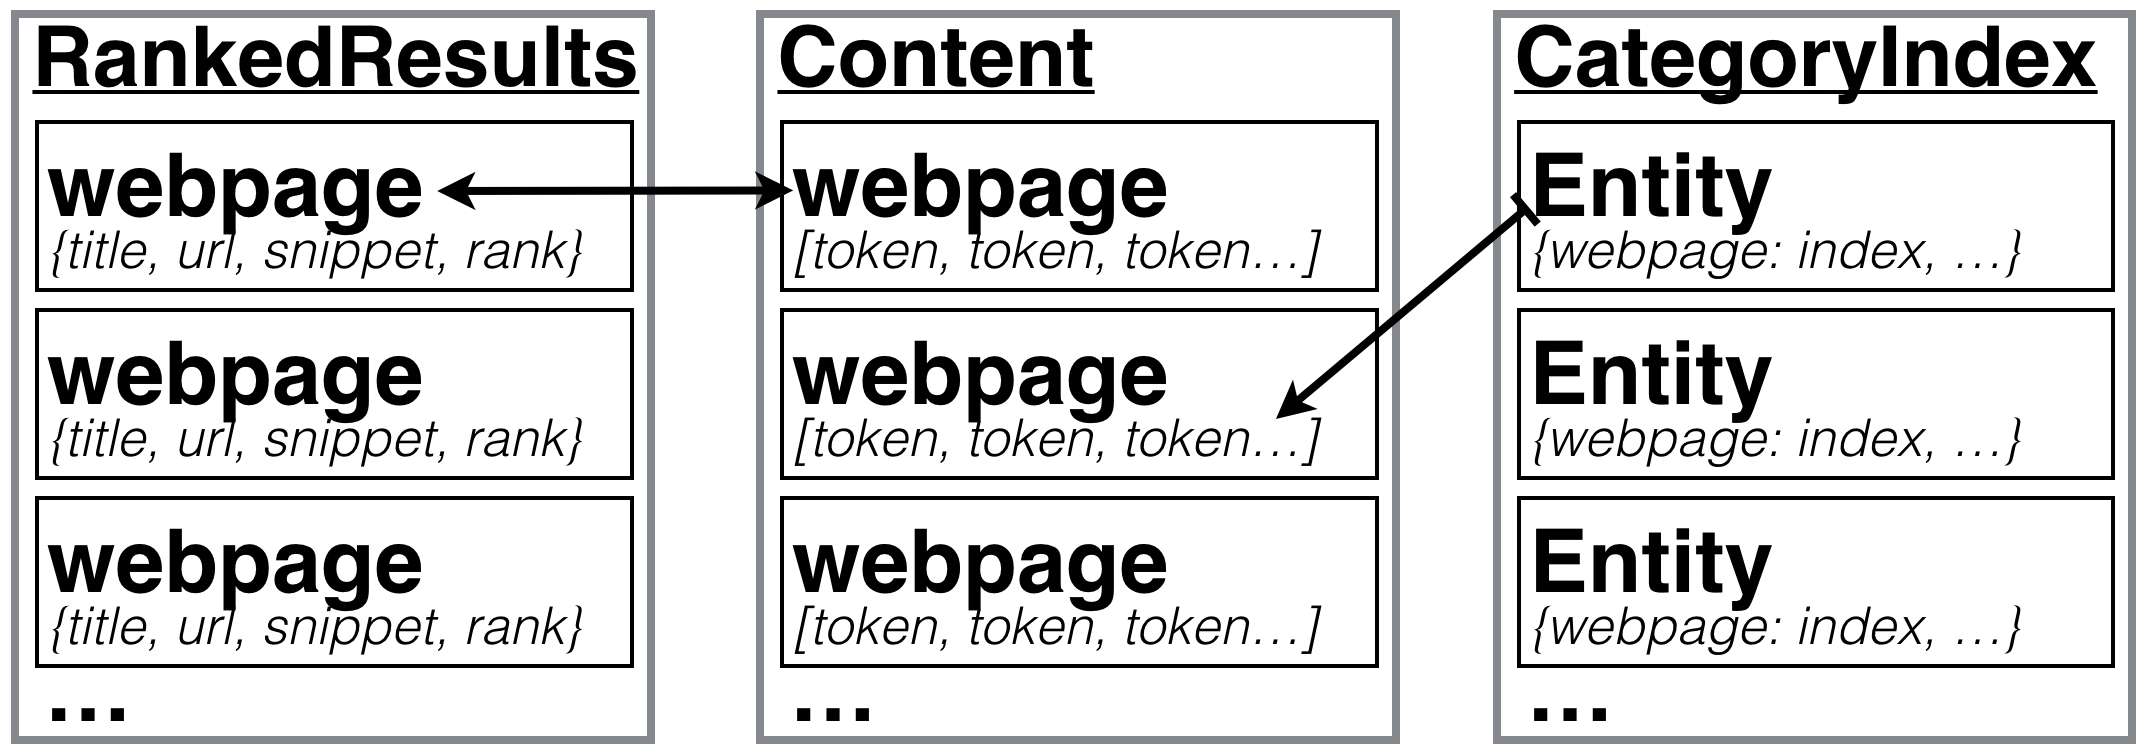
\includegraphics[width=0.5\columnwidth]{Chapters/SearchScape/figures/ds.png}
    \caption[The three data objects produced in the SearchScape back-end component.]{The three data objects produced in the SearchScape back-end component, and passed to its front-end component to enable interactive information exploration. The arrows show the mapping relations between elements in different object.}
    \label{fig:ds}
\end{figure}


\begin{enumerate}
   
    \item \textbf{RankedResults}. The ranked search results retrieved from the Microsoft Bing Web Search API, containing the top 50 results for the given query. Each result contains the rank, URL, title, and a short text snippet from the webpage. 
    
    \item \textbf{WebpageContent}. An index that contains an array of tokenized main content of each webpage in the search results.
    
    \item \textbf{CategoryIndex}. The identified category and its list of entities as described in the previous subsections. Each entity has an inverted-index file\cite{baeza1999modern} of webpages and indices of where the entity was mentioned in WebpageContent. 
\end{enumerate}

Figure~\ref{fig:ds} shows the mapping relations between the three data objects. The addition of CategoryIndex and WebpageContent to traditional web search engines enabled the SearchScape front-end to perform the following complex associations in real-time: 

\begin{itemize}

    \item Filter the RankedResults by using the CategoryIndex to find the list of webpages that mentioned a specific entity of interest, and calculate its proportion of mentions.
%    \item Calculate the proportion of webpages in RankedResults that mentioned a specific entity of interest by counting the length of the filtered RankedResults and its original length.
    \item List sentences that mentioned a specific entity of interest by using the CategoryIndex to find webpages and token indices where the entity was mentioned, and extract sentences from WebpageContent.
    \item Count word frequencies in the extracted sentences to find keywords that frequently co-occur with the entity of interest.
\end{itemize}

We will describe in detail how the SearchScape interface utilize these operations to enable interactive data exploration in the next subsection. 


\begin{figure}
    \centering
    \frame{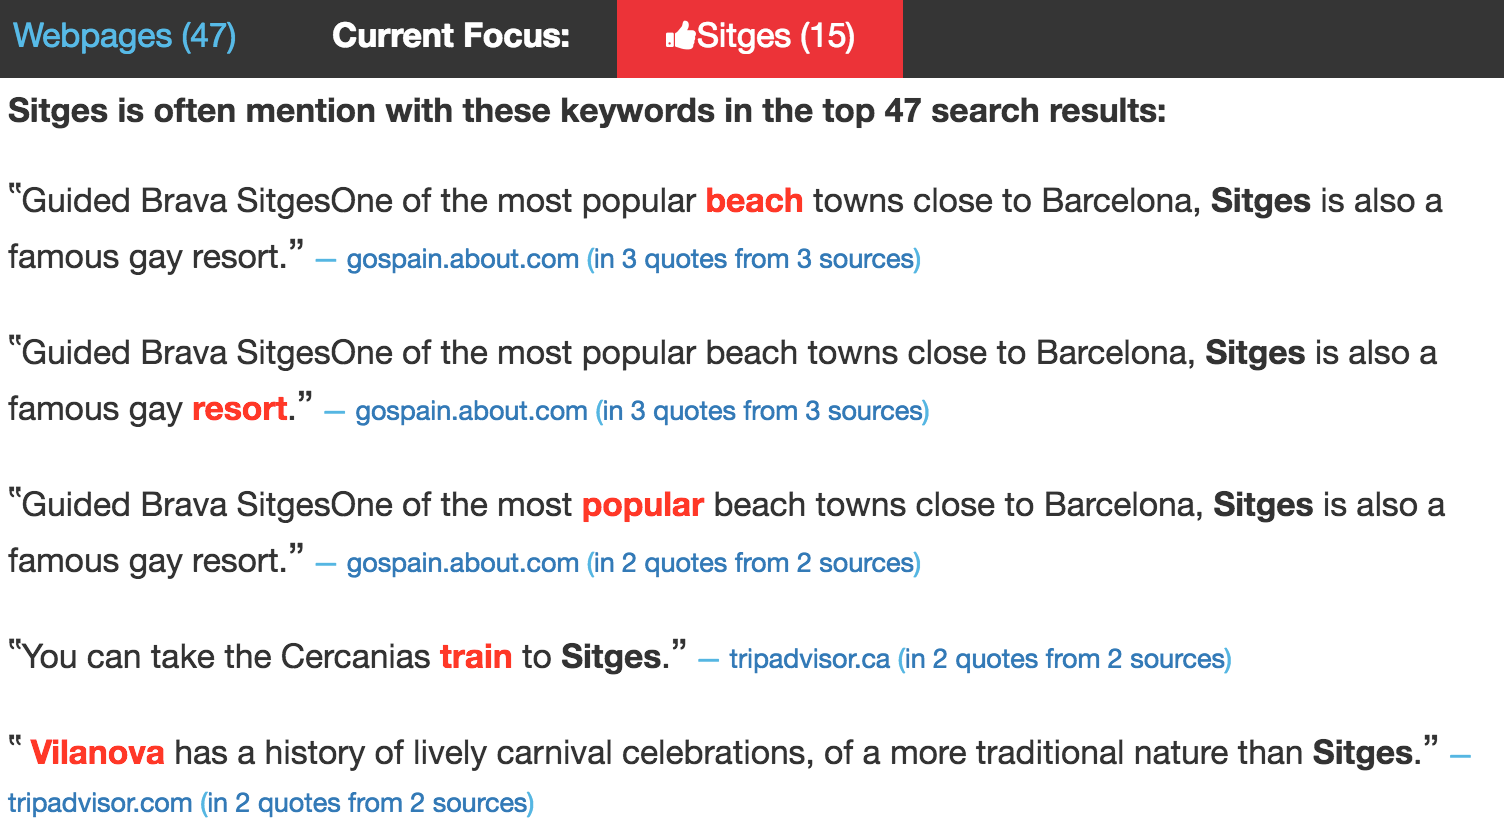
\includegraphics[width=0.6\columnwidth]{Chapters/SearchScape/figures/keywords.png}}

    \vspace{0.5mm}
    
    \frame{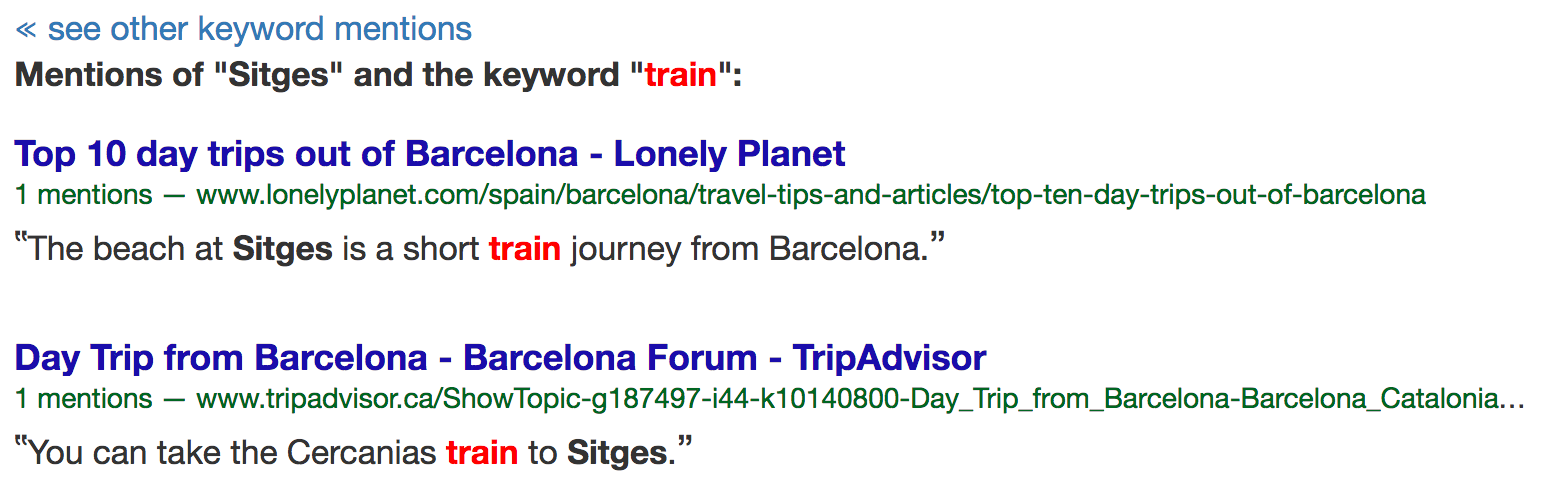
\includegraphics[width=0.6\columnwidth]{Chapters/SearchScape/figures/keywords2.png}}
    
    \caption[Explore mentions and frequently co-occurring words of an concept.]{The searcher clicked on ``Sitges'' from the result page of ``\emph{day trips from Barcelona}'' to explore its mentions grouped by frequently co-occurring keywords, such as \emph{beach}, \emph{resort}, and \emph{train}.}
    \label{fig:keywords}
\end{figure}



\subsection{Interactive Search Landscape}

Using the structures identified by its back-end components, the SearchScape interactive front-end interface augments traditional ranked list search results both to provide a quick overview of the information landscape, and to enable deep user interaction for exploring important subtopics specific to the current query. 

%
%\begin{figure}
%    \centering
%    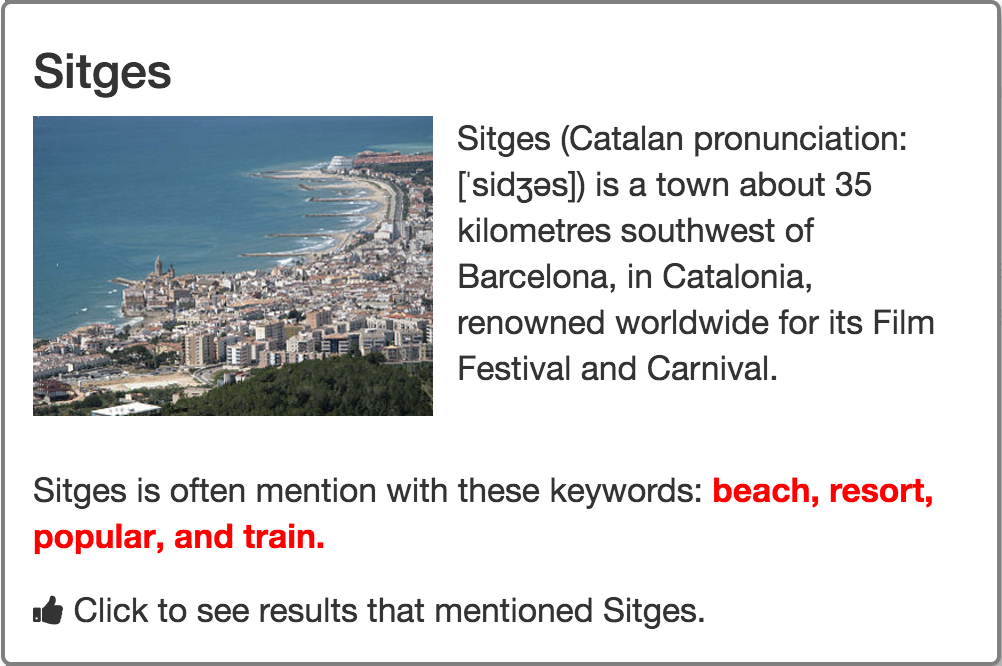
\includegraphics[width=0.6\columnwidth]{Chapters/SearchScape/figures/preview.png}
%    \caption{Hovering over an extracted item in SearchScape allows searchers to read a short definition of the concept and frequently co-occurring keywords. Here, the searcher hovered over ``Sitges'' from the search result page of ``\emph{day trips from Barcelona}''.}
%    \label{fig:preview}
%\end{figure}


SearchScape supports many key tasks defined in Shneiderman's task taxonomy of information visualization \cite{shneiderman1996eyes}, such as \emph{overview}, \emph{zoom}, \emph{filter}, and \emph{details-on-demand}. The interface consists of a Structure Panel on the left, and a Document Panel on the right (Figure~\ref{fig:flow}, left). When a new search results is loaded, the Structure Panel on the left displays an \emph{overview} of the current information space using the distribution information of items in the identified category, and the Document Panel on the right lists webpages in the search results. Similar to many commercial search engines, the Document Panel shows the title, URL, and a short snippet related to the query terms for each webpage in the search results. Even though SearchScape can automatically identify key concepts from the search results, exploratory searchers might not be familiar with the extracted concepts, especially in early stages of the exploratory search process. Therefore, SearchScape allows searchers to \emph{demand-for-details} when needed by hovering over the items to see short descriptions of the concepts from external knowledge bases (Figure~\ref{fig:flow}, left). In addition, SearchScape also extracts a list of keywords that frequently co-occur with the concept of interest in the search results using the inverted-index file. When the searchers discovered an interesting item, they can \emph{filter} the Document Panel by clicking the item of interest (Figure~\ref{fig:filter}, left). A focus tab will appear on the top of the Document Panel to indicate the the current items of interest (Figure~\ref{fig:filter}, center), and the Document Panel will re-rank webpages that mentioned the item to the top of the list, as well as update the short descriptions to show parts of each webpage that mentioned the item. Instead of looking through the filtered search result list, searchers also have the option to \emph{zoom-in} to the current focused item by clicking on the focus tab to see sentences in the search results that mentioned the item of interest, grouped by frequently co-occurred keywords (Figure~\ref{fig:keywords}).

\begin{figure}
    \centering
    \frame{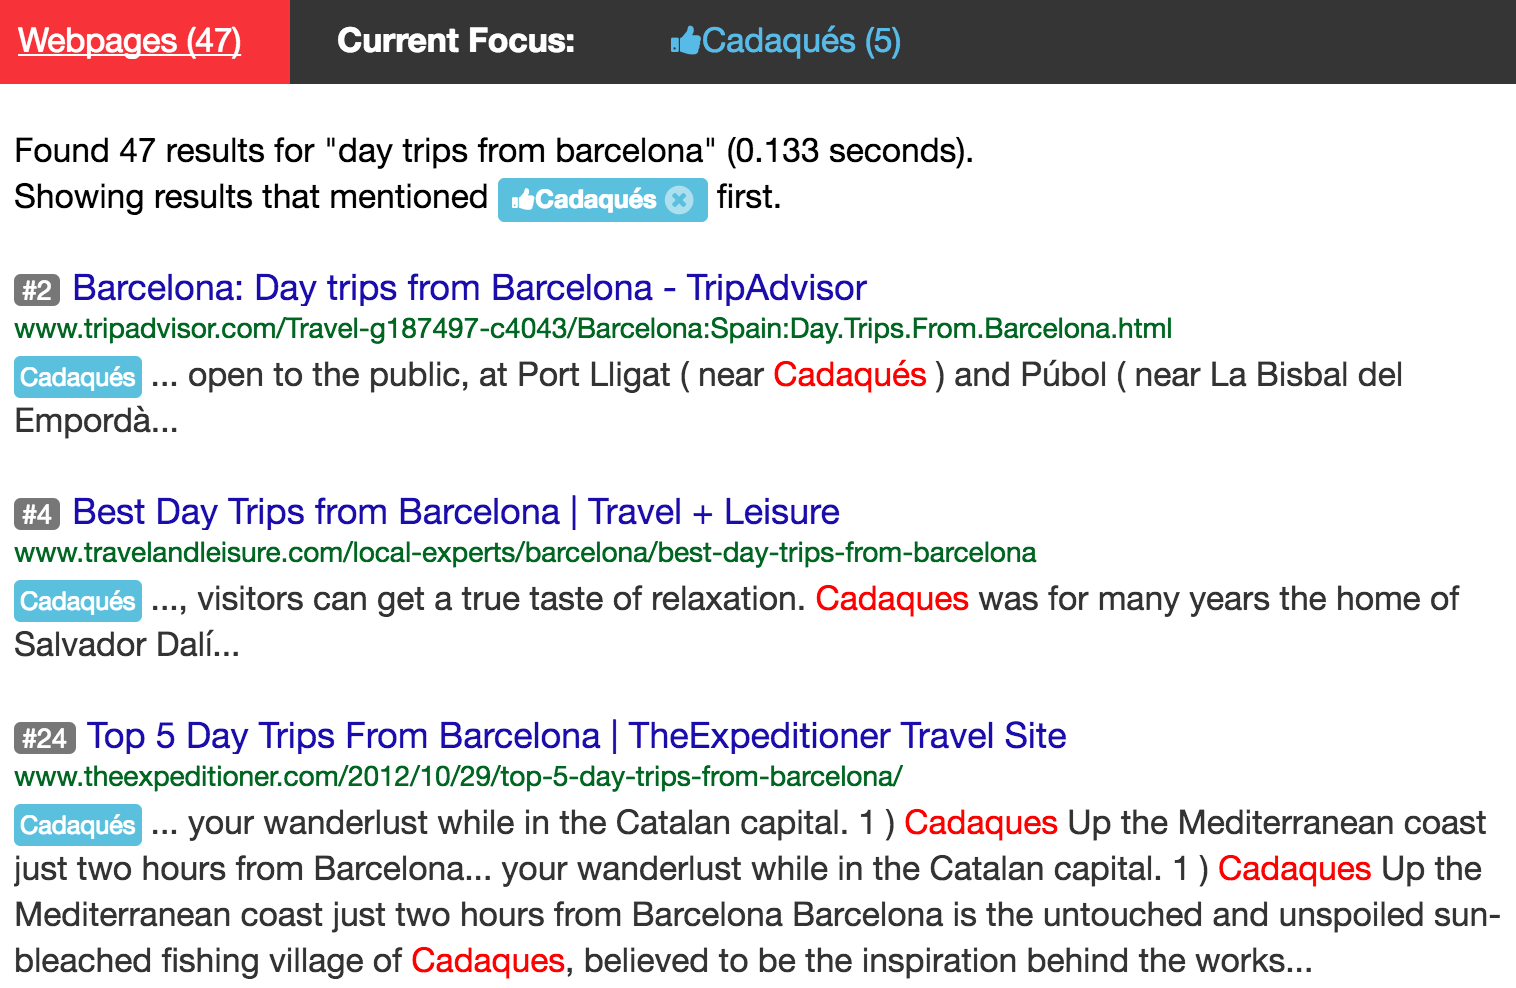
\includegraphics[width=0.6\columnwidth]{Chapters/SearchScape/figures/filter.png}}
    \caption[Filtering the search results using ``Cadaqu\'es'' from the result page.]{The searcher filtered the search results using ``Cadaqu\'es'' from the result page of ``\emph{day trips from Barcelona}''. Notice the snippets are updated to show relevant parts of each webpage.}
    \label{fig:filter}
\end{figure}


To give a sense of how an exploratory searcher might use SearchScape, we will use Figure~\ref{fig:flow} as an example scenario. In our scenario, the user searched for ``\emph{day trips from Barcelona}'', the SearchScape back-end analyzed sources in the search results and identified the Freebase category \emph{GeographicLocations} as the most useful category for the current task. The list of ranked search results are presented to the user in the Document Panel, and a list of different destinations and how frequently each of them are mentioned by different sources are presented in the Structure Panel. By examining the items in the \emph{GeographicLocations} category, the user quickly gained an overview of how many different destinations are in the search results, and how popular each of the choices are (Figure~\ref{fig:flow}, left). The user then proceeded to explore the different choices in the Structure Panel by hovering over each of the items. The user noticed that the destination ``Sitges'' is mentioned in a third of the sources, and is also frequently mentioned with keywords that matched with his or her interests, such as ``\emph{beach}'' and ``\emph{resort}''. To access more information about Sitges, the user clicked on Sitges to surface sources that mentioned Sitges (Figure~\ref{fig:flow}, center. Figure~\ref{fig:filter}), and also directly explored sentences from different sources that mentioned both ``Sitges'' and ``beach'' (Figure~\ref{fig:flow}, right. Figure~\ref{fig:keywords}).


\section{Evaluation}



We evaluated SearchScape through two studies aimed at assessing the coherence of the identified structures and the usefulness of the interface, respectively. For the first study, we compared structures generated for 50 different search queries from an exploratory search database \cite{potthast2013exploratory,Hagen:2016:WSA:2854946.2854969} using both SearchScape and Carrot2 \cite{stefanowski2003carrot}, a search result clustering system.
For the second study, we recruited 210 unique participants from Amazon Mechanical Turk for a user study \cite{kittur2008crowdsourcing}.
Three diverse search scenarios were designed as between-subject conditions in Study 2 to evaluate the usefulness and generalizability of SearchScape. 
To further examine whether providing distribution information is actually beneficial to searchers,
we grouped participants under each of search scenario into two front-end conditions to test the effects of hiding and exposing distribution information of the extracted items (Figure~\ref{fig:conds}). In the following subsections, we will describe the two studies in detail.

\begin{figure}
    \centering
    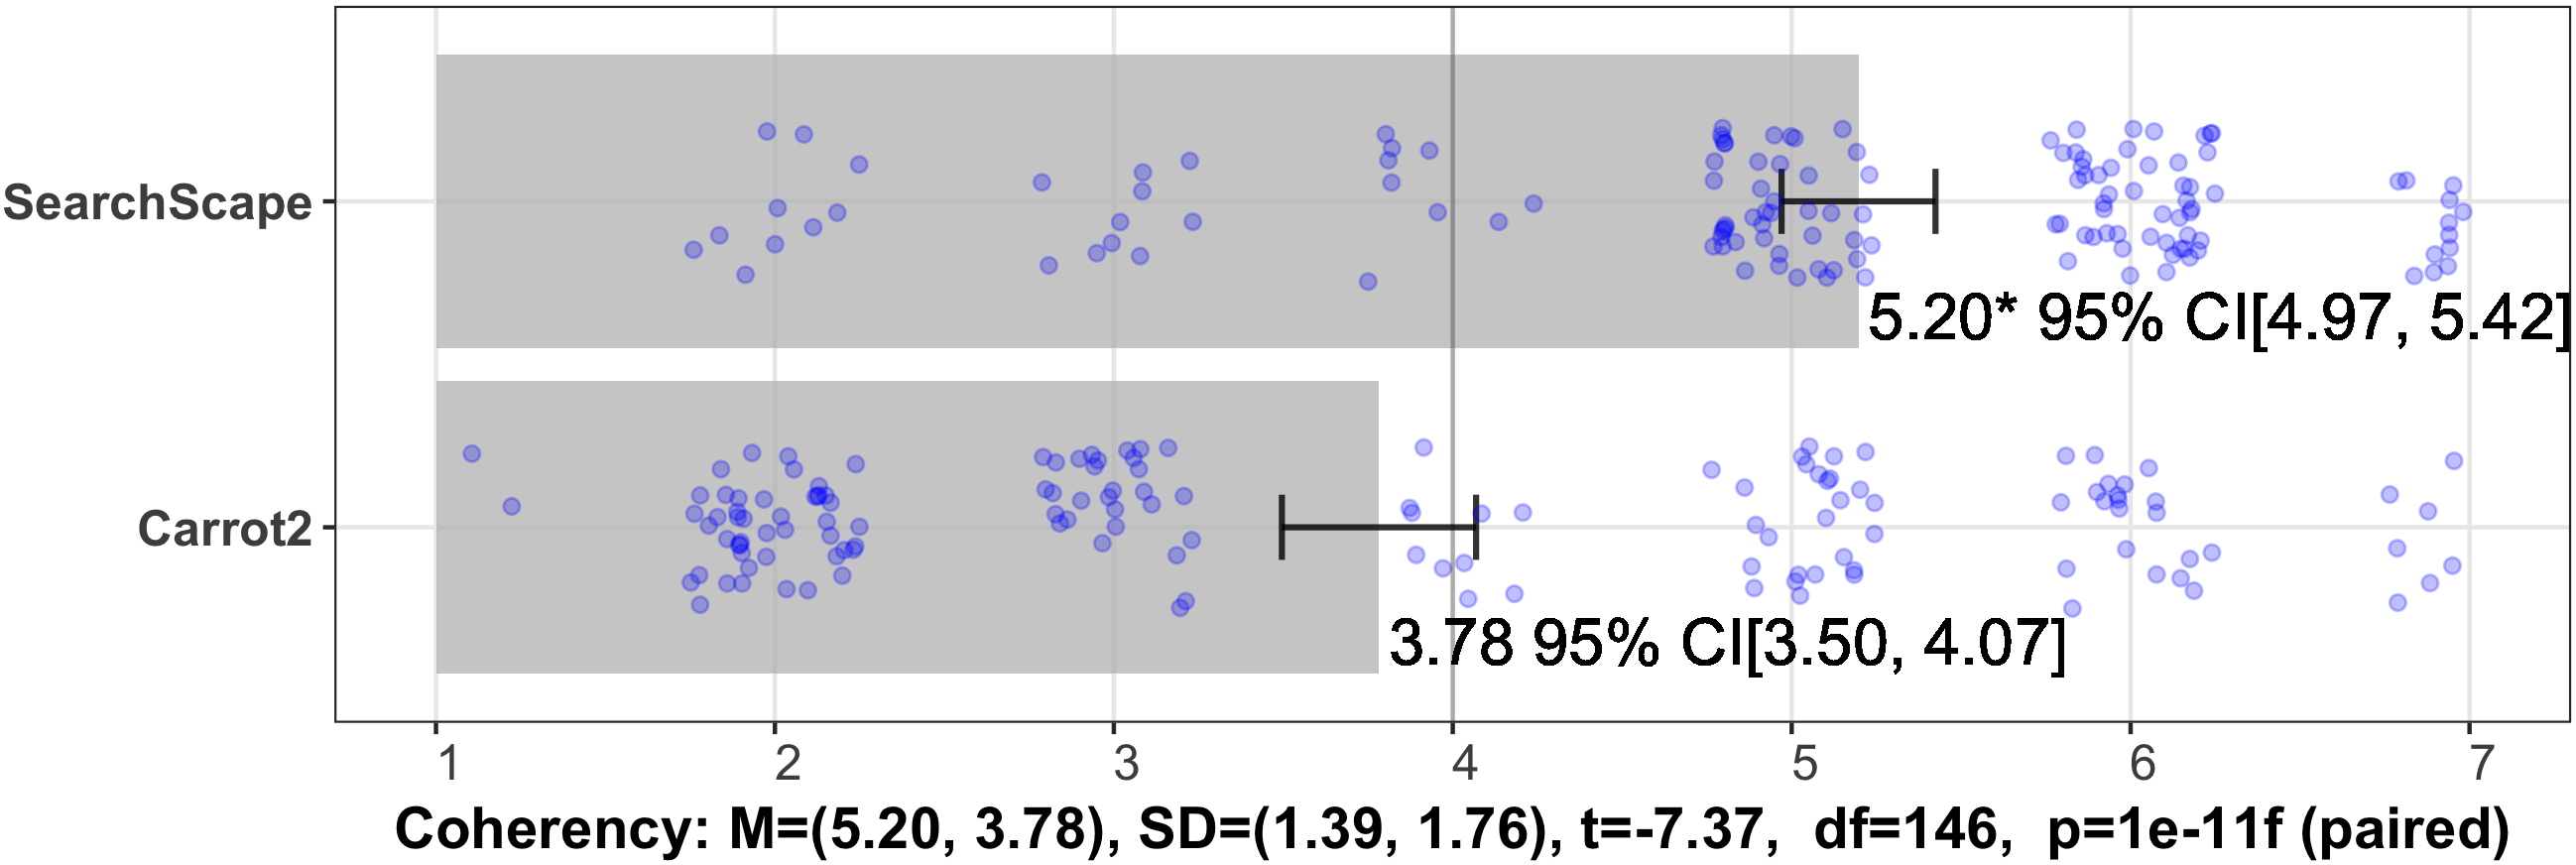
\includegraphics[width=0.6\columnwidth]{Chapters/SearchScape/figures/coherence_label.png}
    \caption[SearchScape structures were found to be strongly coherent, and significantly more coherent compared to Carrot2 based on paired t-test.]{Using 7-point Likert scales,  
    SearchScape structures were found to be strongly coherent (M=5.20*, 95\% CI[4.97, 5.42]), and significantly more coherent compared to Carrot2 (M=3.78*, 95\% CI[3.50, 4.07]) based on paired t-test (N=147, t=-7.37, df=146, p<0.001). The error bars indicate confidence intervals.
        }
    \label{fig:coherence}
\end{figure}

\begin{table}
\small
    \centering
    \begin{tabular}{l}
    \hline
        Statements \\
        \hline
        
        S1. Seeing the \textbf{list of items} on the left is useful \\
       
        S2. The \textbf{distribution/rank} each item is on the left is useful \\
        
        S3. Clicking on an item to see \textbf{webpages} that \textbf{mentioned} it is useful \\
        
        S4. Seeing \textbf{keywords} often \textbf{mentioned} together with the items is useful \\
        
        S5. For complex searches, this is an \textbf{improvement} to current interfaces \\
        
        S6. I would \textbf{prefer} it if my search engine have these extra features \\
        
        S7. I think the extra features would help me \textbf{find better} information \\
        
        S8. The interface is a \textbf{distraction} or makes searching more \textbf{stressful} \\
        
        \hline
        
    \end{tabular}
    \caption[Full statements rated by the participants.]{Full statements rated by the participants. Statements were not stylised in the survey.}
    \label{tab:statements}
\end{table}



\begin{table}
\small
    \centering
    \scriptsize
    \begin{tabular}{r | l l | l l | l l}

    & \multicolumn{2}{c|}{Barcelona} & \multicolumn{2}{c|}{Guacamole} & \multicolumn{2}{c}{Guggenheim} \\ 
        Stmt. & DIST & RANK & DIST & RANK & DIST & RANK   \\
        \hline
        
        
        S1 & 
        \textbf{4.35}[4.11, 4.60] & 4.12[3.82, 4.43] &  
        \textbf{3.97}[3.99, 4.66] & 3.86[3.69, 4.42] & 
        4.22[3.88, 4.57]& \textbf{4.36}[4.08, 4.64]\\
        
        S2 &
        \textbf{4.32}[4.02, 4.63]\textsuperscript{\tiny *} & 3.82[3.45, 4.19] &
        3.89[3.45, 4.33] & 3.89[3.53, 4.26]& 
        4.28[3.93, 4.63] & \textbf{4.44}[4.20, 4.69] \\
        
        S3 &
        \textbf{4.19}[3.89, 4.50]& 4.09[3.78, 4.40]&
        \textbf{4.11}[3.70, 4.51]& 4.08[3.69, 4.47]&
        4.28[3.96, 4.60] & 4.28[3.99, 4.57] \\
        
        S4 &
        \textbf{4.39}[4.12, 4.65] & 4.09[3.74, 4.44]&
        \textbf{3.89}[3.42, 4.37]& 3.76[3.35, 4.17]&
        4.03[3.65, 4.40] & 4.03[3.71, 4.35] \\
        
        S5 &
        \textbf{4.19}[3.89, 4.50]\textsuperscript{\tiny **} & 3.52[3.15, 3.88]&
        4.03[3.62, 4.44]& 4.03[3.65, 4.41]&
        3.94[3.54, 4.35] & \textbf{4.17}[3.86, 4.47]\\
        
        S6 &
        \textbf{4.19}[3.87, 4.51]\textsuperscript{\tiny *} & 3.58[3.20, 3.95]& 
        \textbf{3.76}[3.32, 4.20] & 3.46[3.02, 3.89] &
        \textbf{3.83}[3.42, 4.24] & 3.78[3.43, 4.12]\\
        
        S7 &
        \textbf{3.21}[2.84, 3.58]\textsuperscript{\tiny *} & 2.60[2.26, 2.95]&
        \textbf{3.00}[2.59, 3.41]& 2.70[2.32, 3.09]&
        3.03[2.61, 3.45] & 3.03[2.67, 3.38] \\
        
        \hline
        
        \textbf{Aggr.} &
        \textbf{4.15}[4.03, 4.27]\textsuperscript{\tiny ***} & 3.69 [3.55, 3.83]&
        \textbf{3.81}[3.65, 3.97] & 3.68[3.53, 3.84]&
        3.95[3.80, 4.09]& \textbf{4.01}[3.89, 4.14]\\
        
        \hline
        
        S8 &
        \textbf{2.45}[1.92, 2.99] & 2.79[2.35, 3.23]&
        \textbf{2.19}[1.77, 2.61]& 2.49[2.03, 2.94]&
        \textbf{2.28}[1.86, 2.70] & 2.39[1.94, 2.83] \\
        \hline
        
        \textbf{N} & 31 & 33 & 37 & 37 & 36 & 36 \\
        

        
    \end{tabular}
    \caption[Survey responses under different tasks and conditions.]{(Full statements in Table~ \ref{tab:statements}) Survey responses (mean and 95\% confidence interval) under different tasks and conditions using a 5-point Likert scale. A score of 5 indicates strong agreement with the statement, and a score of 1 indicates strong disagreement. Confidence intervals above 3 indicates significant agreement. Asterisks indicate significant differences between conditions under independent t-test.  \textsuperscript{\tiny *}p $\boldsymbol \le$ 0.05,\textsuperscript{\tiny **}p $\boldsymbol \le$ 0.01, \textsuperscript{\tiny ***}p $\boldsymbol \le$ 0.001}
    \label{tab:survey}
\end{table}



\subsection{Study 1: Automatic Structuring}

To evaluate the quality of the structures produced by SearchScape, we compare it against the open source search results clustering system Carrot2 \cite{stefanowski2003carrot}, which produces interpretable names for each of its clusters. To cover a wide variety of search topics and scenarios, we randomly selected 49 queries from different topics found in a exploratory search database that contains a total of 150 search tasks derived from
the TREC Web track topics of the years 2009 to 2011 \cite{Hagen:2016:WSA:2854946.2854969}. The queries are collected from participants conducting exploratory search for the 150 search tasks in a lab setting \cite{potthast2013exploratory}. We submit each of the 49 queries to both SearchScape and Carrot2 and obtained a total of 98 search result structures. Finally, we present each of the task descriptions, queries, and the pair of structures to 3 crowdworkers. For each structure, we asked the crowdworkers to rate the statement ``\emph{Items in the list are of the same type}'' using a 7-point Likert-scale ranging from Strongly Disagree (1) to Strongly Agree (7), and a score of 4 indicates neutral.

        


%comprehensiveness of the identified structures, we manually compiled gold-standard structures for the two exploratory search tasks by reading through the 50 results for each of the two queries and extracting the destinations and ingredients, respectively. We then used the gold-standard labels to evaluate both the precision and recall rate of the SearchScape categories and items. To account for prominence, we weighted the recall rate using the number of results that mentioned each item in the gold-standard labels. 


\subsubsection{Results}


As shown in Figure~\ref{fig:coherence},
participants agreed strongly that SearchScape produced structures that were coherent (M=5.20*, 95\% CI[4.97, 5.42]).
When compared side-by-side against structures produced by Carrot2, crowdworkers rated SearchScape as more coherent (M=(3.78 vs 5.20), SD=(1.76, 1.39)). This difference was significant based on a paired t-test (N=147, t=-7.37, df=146, p=1e-11f < 0.001). The results suggest that for a wide variety of exploratory search scenarios, SearchScape can produce structures more coherent than traditional search result clustering approaches. %In Study 2, we examine if the structures were actually beneficial to searchers using the interactive SearchScape interface. Further, we explore if exposing distribution information with these coherent structures has a positive effect to searchers.

%As shown in Figure~\ref{fig:pr}, for the Barcelona task, SearchScape identified the Freebase \emph{GeographicLocations} category, which initially covered 45\% of the entities in the gold-standard, and has a precision rate of 81\%. Expanding the category using the Word2Vec model raised the recall rate from 45\% to 68\%, and only lowered the precision rate by 1\%. For the Guacamole task, SearchScape identified the NELL \emph{AgriculturalProducts} category, which initially already covered 66\% of the gold-standard labels, but at with a lower precision rate of 64\%.  After expanding the category using the GloVe model, the coverage was further increased to 72\%, but at the cost of decreasing the precision rate to 56\%. In both scenarios, SearchScape reached around 70\% recall rate, which covered the majority of concepts that were mentioned in at least two sources due to long-tail effects (around half of the gold-standard labels were items only mentioned once in the search results). We also examined cases where SearchScape included concepts that were not in the gold-standard, and discovered the main cause being some sources contained information irrelevant to the query. For example, webpages that contained guacamole recipes but also recipes of other dishes, or webpages that contained information about day trips from Barcelona, but also multi-day plans that reached places too far for day trips. 


%\begin{figure}
%    \centering
%    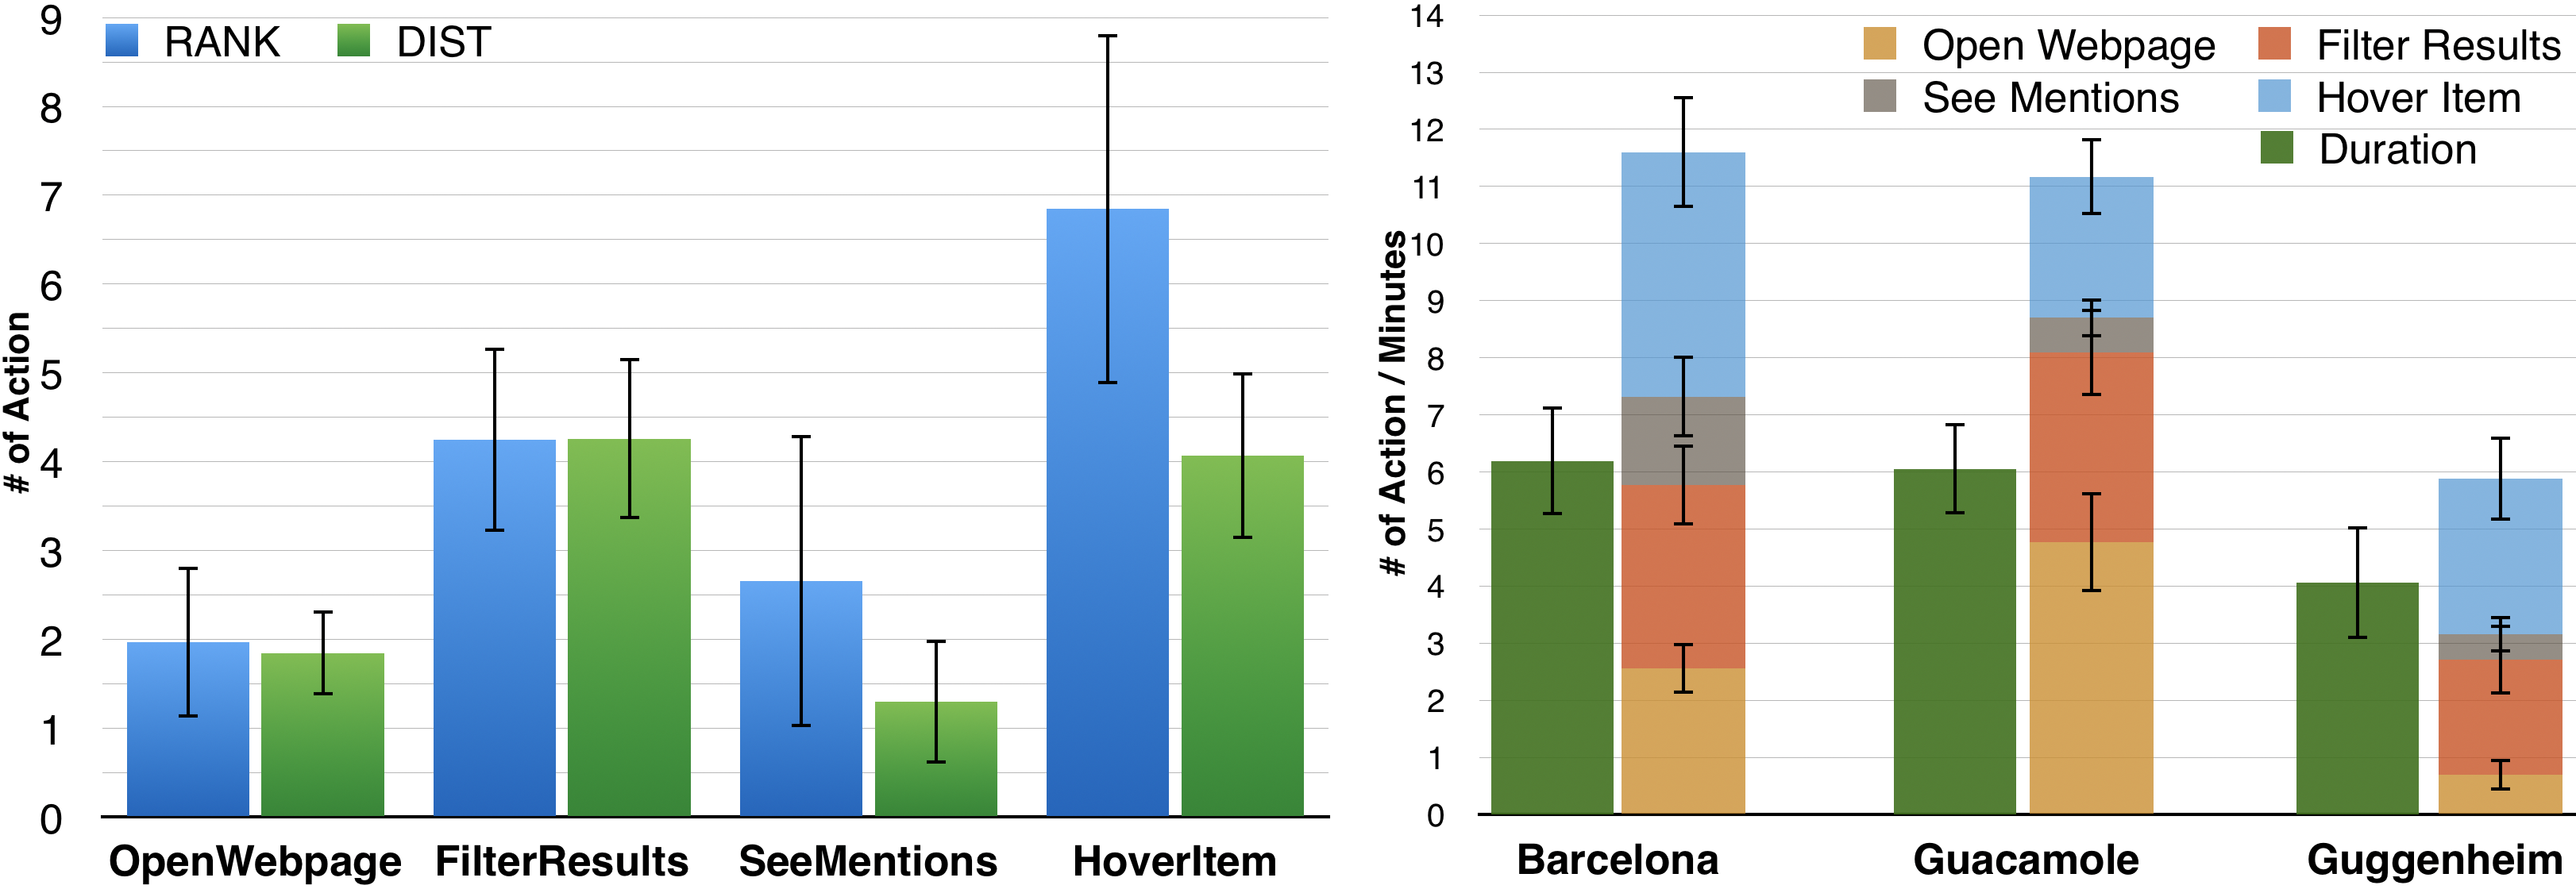
\includegraphics[width=0.96\columnwidth]{Chapters/SearchScape/figures/time.png}
%    \caption{Average number of actions each participant performed in the two exploratory tasks (left). Average number of actions participant performed and average duration spent under different tasks (right).}
%    \label{fig:time}
%\end{figure}


\begin{figure}
    \centering
    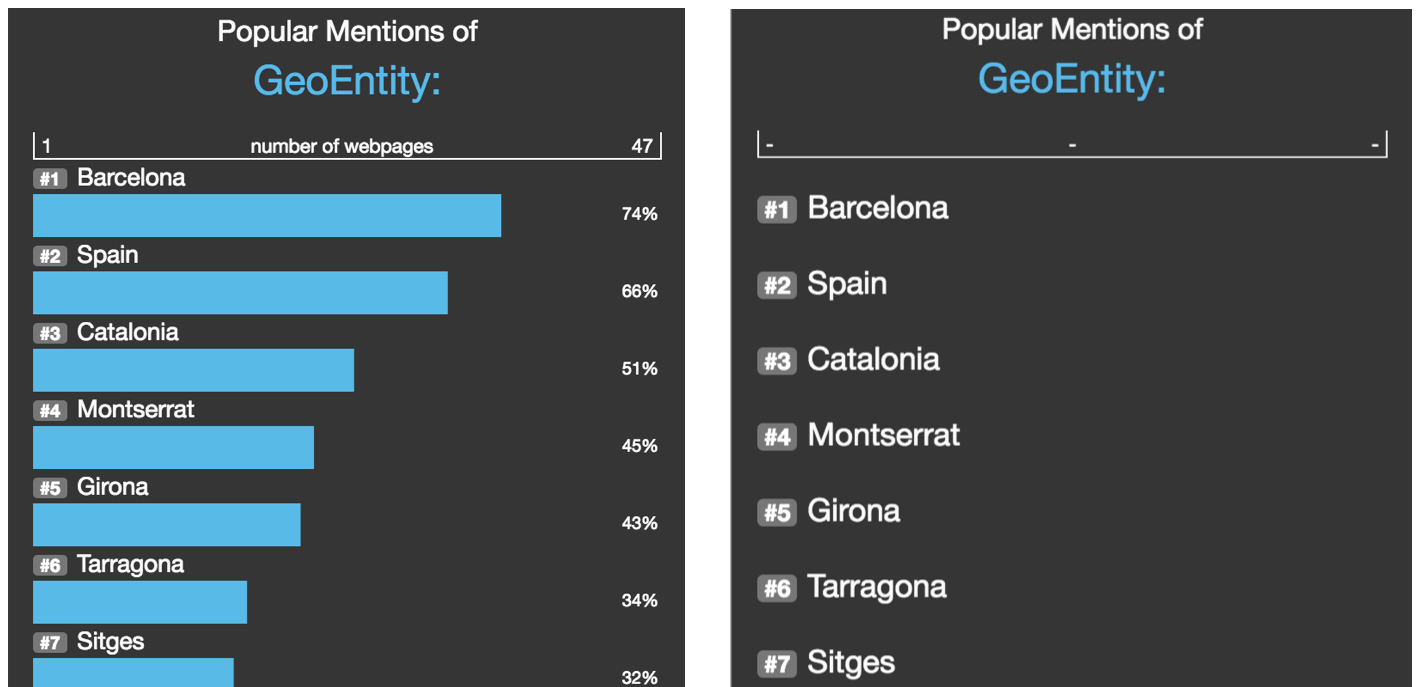
\includegraphics[width=0.6\columnwidth]{Chapters/SearchScape/figures/conds_short.png}
    \caption[A baseline system used in the SearchScape study.]{The DIST condition (left) shows the proportion of results mentioned each items in the category. The RANK condition (right) hides the distribution information, but still shows the ranking of each item.}
    \label{fig:conds}
\end{figure}



\subsection{Study 2: Exploratory Search}

Automatically identifying important structures and displaying distribution information are the two key components that differentiate SearchScape from traditional Web search interfaces and previous work. In order to evaluate the usefulness of the SearchScape interface, and more specifically, the benefits of exposing structural and/or distribution information to searchers, we conducted a user study with 210 unique participants recruited from Amazon Mechanical Turk (age between 18 and 68, M=35, SD=11, 57\% male and 43\% female, mostly from the US) \cite{kittur2008crowdsourcing}.

The experiment was a 3x2 between subjects design, with participants randomized into one of the three different search scenarios and one of the two interface conditions (rank+distribution or rank only) as shown in Figure~\ref{fig:conds}. The \textbf{DIST} condition consisted of all features described in the previous section, which showed both the ranks and proportions of webpage mentions of the items using text labels and horizontal blue bars of different lengths. The \textbf{RANK} condition consisted of all the same interactive features, but hid the distribution of items by only showing their ranking. 
During the study, participants first filled out a pre-survey about their demographic information, we then presented each participant with their assigned search tasks.
%In the first part of the study, we provided the participants with only the top search results of each task without the SearchScape features. For the \textbf{Barcelona} task, we provided the top-1 search results from the Bing Web Search API, which contains seven day trip destinations from Barcelona.\footnote{touropia - 7 Great Day Trips from Barcelona, http://www.touropia.com/day-trips-from-barcelona/} For the \textbf{Guggenheim} task, we also provided the top-1 search result, which contains the correct answer in the second paragraph.\footnote{Wikipedia - Solomon R. Guggenheim Museum, https://en.wikipedia.org/wiki/Solomon\_R.\_Guggenheim\_Museum} For the \textbf{Guacamole} task, we provided the top-7 search results, which, in total, contains seven recipes. We asked the participants to review top results and answer the tasks the best they can. This part of the study aimed to ensure that they are aware of the uncertainty in the tasks (i.e., multiple choices exist), and motivate them to verify and explore different the options in the next part of the study \cite{kules2008creating}. In the second part of the study, 
They then watched a 70 second video tutorial introducing the features of SearchScape according to their front-end conditions. They were then asked to conduct the assigned search tasks using SearchScape. As they interact with the interface, we recorded their actions for further analysis. Finally, we collected their opinions about SearchScape in a post-survey (Table \ref{tab:survey}). 

\subsubsection{Search Scenarios}

Creating tasks to effectively evaluate exploratory search systems is itself a challenging task \cite{kules2008creating,white2006report}. Challenges include finding topics that are unfamiliar yet still relatable for the participants and motivating participants to explore and evaluate different options. We designed two exploratory tasks of different complexity, following the task design suggestions outlined in \cite{kules2008creating}, such as providing ample imaginative context, and being specific about the information necessary for their assigned search task. In addition, we also included one fact-finding task to see if the additional features of our interface would interfere or cause annoyance in non-exploratory scenarios. For each task, participants were given a fixed query that we have fetched and indexed in advance using the back-end of SearchScape. Below are the three tasks we utilized in this study and their corresponding queries:

\begin{itemize}
    \setlength\itemsep{0.0em}
    \item \textbf{Barcelona}. ``\emph{You have a friend who's planning a day trip from Barcelona, and you want to help her figure out 3 destinations that you considered the best options. Give a short explanation about why you picked each of the destinations.}'' \textbf{Query}: ``\emph{day trips from Barcelona}''
    \item \textbf{Guacamole}: ``\emph{You are in charge of making guacamole for a party you and your friends are hosting. You've decided to do some searching online to find 3 recipes you like the most.  Give a short explanation about why you picked each of the recipes.}'' \textbf{Query}: ``\emph{guacamole recipes}''
    \item \textbf{Guggenheim}: ``\emph{You need to find out who designed The Guggenheim Museum in New York City for a school report, and you decided to search the Internet for the answer. Give a short explanation for how you found the answer.}'' \textbf{Query}: ``\emph{who designed the Guggenheim Museum?}''
\end{itemize}

The three tasks were designed with the following factors in mind. The \textbf{Barcelona} scenario promotes objective decision making based on the information presented, since we did not specify a persona for the person participants were gathering information for. Conversely, the \textbf{Guacamole} scenario promotes subjective decision making, since the participants are searching for recipes for themselves.
%We therefore expected participants to benefit more from the distribution information in the first task, and hope the overview provided by the structures can help participants to find unique options that they preferred.
In addition, the relationship between the identified structures and information needs also differs. SearchScape identified a list of \emph{geographic locations} for the \textbf{Barcelona} query, which were mostly competing \emph{places} for day trip destinations, whereas for the \textbf{Guacamole} query, SearchScape identified \emph{agriculture products}, which contained mostly composable \emph{ingredients} of different recipes.
%We considered the \textbf{Barcelona} task to be our most complex task, containing unfamiliar choices with multiple attributes (i.e., activities for different destinations), and expected most participants to actively engage in exploratory search during the study. On the other hand, \textbf{Guacamole} task was designed to be a simpler exploratory task, where participants were likely already familiar with the ingredients of different recipes before the study.
Finally, we included the simple fact-finding \textbf{Guggenheim} task to see if participants find the extra features overwhelming or detrimental for finding a single correct answer.

\begin{figure}
    \centering
    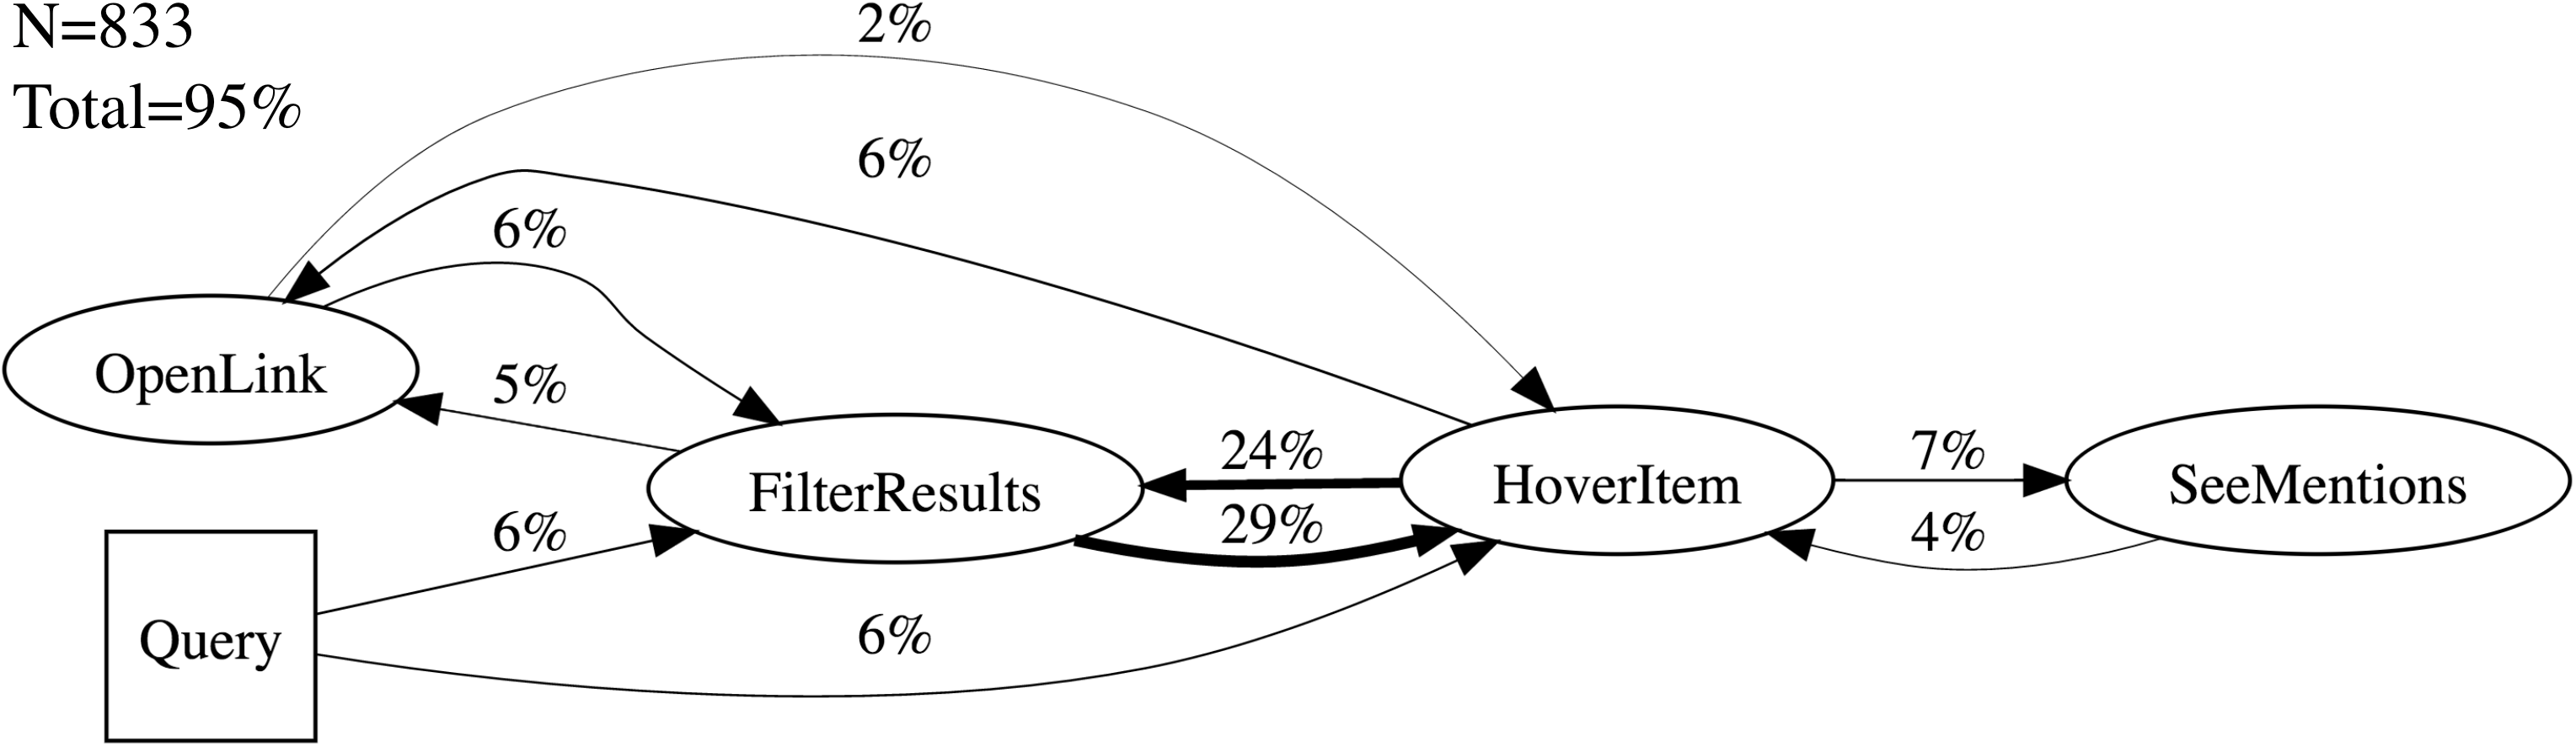
\includegraphics[width=0.7\columnwidth]{Chapters/SearchScape/figures/trans.png}
    \caption[Top transitions between different features.]{Top transitions between different features of participants across all conditions.  Around half of the participants started by hovering items, while the other half by filtering the search results.}
    \label{fig:trans}
\end{figure}


\section{Results and Discussion}


\subsection{Behavior}

%On average, participants performed 11.5 actions in 6 minutes for the two exploratory tasks, and 6 actions in 4 minutes for the fact-finding task (Figure~\ref{fig:time}).
%Participants were also actively engaged with the features provided by SearchScape (Figure~\ref{fig:time}, left).
%On average, participants in the RANK condition performed more HoverItem and SeeMentions actions, but the differences were not significant. 
%Participants also used the structures to gain an overview of the information space. 
SearchScape augments traditional search interfaces with a interactive information landscape. First, we examine whether participants were actually using the added features. 
Figure~\ref{fig:trans} shows the top 10 transitions between different SearchScape features, and
participants almost always explored the overview information in the Structure Panel first, instead of opening links from the list of search results directly. Similar findings have been reported in previous work on using a faceted interface to explore a library catalog \cite{kules2009exploratory}.


% \subsubsection{Results: Searcher Preferences}
% Table \ref{tab:survey} shows the eight survey questions and responses we collected. The first four questions were each about a different feature of SearchScape. The next three questions were about their overall opinions about SearchScape, including two questions comparing SearchScape to traditional web search interfaces. Finally, we asked the participants whether the additional features of SearchScape caused distractions or stress. In general, participants responded favorably to both SearchScape conditions, even in the fact-finding \textbf{Guggenheim} task. Comparing the two frond-end conditions, the DIST condition were found to be significantly more useful than the RANK condition, but only in the most complex \textbf{Barcelona} task. Finally, we also coded the answers and general feedback from participants, and we will show representing quotes in the Discussion Section.


\subsection{SearchScape vs Traditional Web Search Interface}

SearchScape augments traditional web search interfaces with structure and distribution information, which enables interactive information exploration. The results of our studies suggested the structure and distribution information helped participants process and navigate large amounts of information efficiently.
Participants were asked to compare SearchScape to their current search engine interfaces using a 5-point Likert scale (Table \ref{tab:survey}, DIST condition). Across three search tasks, participants generally agreed that SearchScape is an improvement to current interfaces (average: 4.2*, 4.0*, 4.0*, respectively, 95\% CI > 3.0), and would prefer it if their search engines also had the extra features (average: 4.2*, 3.8*, 3.8*, respectively, 95\% CI > 3.0). Further, they also agreed that the added features did not cause distraction or stress, even for the fact-finding Guggenheim task (average: 2.5*, 2.2*, 2.3*, respectively, 95\% CI < 3.0). In the general feedback, participants also expressed how SearchScape is an improvement to the current interfaces, and how they felt more organized and/or efficient with the extra features (12.9\%, 5.4\%, and 15.2\% of the participants in the three search tasks, respectively):

%\blockquote{\emph{``It is a more organized way to research at a glance, and saves time that would be spent scanning articles for information.''}}

%\blockquote{\emph{``I did find it to be helpful to be able to search my topic from different angles. The list on the left helped me to re-focus and/or think differently about the topic, if I were struggling to find useful information through my original search...''}}

\blockquote{\emph{I found the interface to be very effective and efficient even while hosting a large amount of information it was easy to wade through the results. When I first watched the video I was skeptical but it really did make finding information much easier to process and understand.}}

We also asked participants about the different SearchScape features (first four questions in Table \ref{tab:survey}), and participants generally agreed that the added features were useful during their search sessions. Of which, using the Structure Panel to quickly drill-down to the different subtopics was the most commonly mentioned feature in the feedback  (19.8\% of participants under DIST and 14.9\% of participants under RANK):

\blockquote{\emph{I like the information on the left. It has all the information i needed without making new searches all of the time. You just have to click on each link to see if it has the new information that you are looking for.}}


These results combined with the behavior logs suggest that participants in our studies were actively using the features provided by SearchScape to complete their tasks, and seemed to consider them improvements to the traditional web search interfaces. In the next subsections, we will examine more closely on how SearchScape performed under different type of search tasks using the three search scenarios we designed. 


\subsection{The Barcelona Scenario}


Of the search scenarios, we consider the Barcelona scenario to be the most complex task of the three. First participants were faced with competing choices that were generally unfamiliar to our participants (i.e., places near Barcelona). In addition, unlike ingredients in a recipe, destinations often have multiple important attributes relevant to the task that participants need to keep track of, such as common activities, or distance from Barcelona. 
For this scenario, SearchScape identified 46 \emph{geographic locations} mentioned in the search results of the query \emph{``day trips from Barcelona''}, and many of which were presented as day trip destinations from Barcelona in the webpages. 

In general, the participants answered favorably on post-survey questions with participants in the DIST condition (the full SearchScape system) responding with an average rating of 4.15* (95\% CI[4.03, 4.27]) across questions regarding the usefulness of SearchScape (Table~\ref{tab:survey}).
In addition, based on independent t-tests, participants in the DIST condition also responded to the survey questions significantly more favorably when compared to participants in the RANK condition, both aggregated (t=4.90, p=1.3e-06) and on four individual questions, suggesting that in this complex scenario, showing the distribution of the items was perceived as significantly more useful (S2, t=2.13, p=0.037), more improvement to the current interface (S5, t=2.78, p=0.007), was more preferred by the participants (S6, t=2.53, p=0.01), and was believed more strongly that they can find better information (S7, t=2.41, p=0.02). Qualitative results also showed similar pattern, with more participants mentioning they found the distribution being useful in the DIST condition then the number of participants in the RANK condition (12.9\% vs 3.0\% of participants): 

\blockquote{\emph{I enjoyed using the interface because for whatever topic you're searching for, it gives you great ``summary'' type results on the left. ... To see percentages helps a lot with pinpointing what you want to find.}}


Some participants in the RANK condition raised concerns about the interface being cluttered and the amount of information was too overwhelming (15.2\% of participants):

\blockquote{\emph{I feel like there is almost TOO much information, making it harder for me to narrow down choices. I could almost see myself spending a few hours just diving deeper into what the best spots really would be. ... with so much info, I'd begin to wonder if I had made the wrong choice.}}

Interestingly, less participants (3.2\%) in the DIST condition (the full SearchScape) mentioned \emph{clutter} or \emph{overwhelming} in their feedback, even though their interface contained more information. This may suggest the counterintuitive potential for extra information to reduce perceived complexity if it promotes a sense of efficacy and understanding of the information space, and may be worth following up in future work.

% Table \ref{tab:survey} shows the eight survey questions and responses we collected. The first four questions were each about a different feature of SearchScape. The next three questions were about their overall opinions about SearchScape, including two questions comparing SearchScape to traditional web search interfaces. Finally, we asked the participants whether the additional features of SearchScape caused distractions or stress. In general, participants responded favorably to both SearchScape conditions, even in the fact-finding \textbf{Guggenheim} task. Comparing the two frond-end conditions, the DIST condition were found to be significantly more useful than the RANK condition, but only in the most complex \textbf{Barcelona} task. Finally, we also coded the answers and general feedback from participants, and we will show representing quotes in the Discussion Section.


\subsection{The Guacamole Scenario}

We designed the Guacamole scenario to be simpler and more subjective than the Barcelona task, but to still have potential for exploration and discovery. For example, searchers might want to find the most authentic recipes or discover unusual ingredients that might not be in the first few search results.  For this scenario, SearchScape identified 59 \emph{agricultural products} mentioned in the search results of the query \emph{``guacamole recipes''}, and many of which were presented as ingredients for making guacamole in the webpages.
 
Participants still responded favorably overall to the SearchScape system with a score of M=3.81* (95\% CI[3.65, 3.97]) averaged across all seven questions on a 5-point Likert scale. However, unlike the Barcelona scenario, participants did not find the DIST condition to be significantly more useful than the RANK condition (Table~\ref{tab:survey}). 
Indeed, many participants considered the Guacamole task to be too simple for the SearchScape interface to be useful (14\% of participants in the Guacamole task, and none in the other two tasks): 

%\blockquote{\emph{``It would be useful for some stuff that is a complex search, but for daily searches not so much. I'd recommend it for research purposes in college or something like that''}}

\blockquote{\emph{I'd definitely use it for more complex searches. For guacamole, no. HAHA. I smoosh avocados, add salt and lemon. No Internet search needed, but I would definitely use it for something more complex.}}

%However, the behavior logs showed that participants in the Guacamole condition performed similar numbers of actions when compared to participants in the Barcelona task, even thought some deemed the task to be too simple for the features to be useful (Figure~\ref{fig:time}, right).
Further analysis of the qualitative feedback, as well as the short explanations for their answers revealed that many were finding recipes that contained uncommon but interesting ingredients, such as \emph{bacon} (only mentioned in 6\% of web pages), \emph{mango} (11\%), or \emph{cumin} (15\%). Their feedback mentioned they discovered these interesting choices from the Structure Panel (19\% of participants in the Guacamole task, and around 12\% in the other two): 


\blockquote{\emph{I like this search engine interface. I like the options that I was able to get in a quick amount of time through those keywords listed on the left. They allowed me to rethink the kind of guacamole recipes I wanted, and exposed me to new types of guacamole recipes. That added to my creativity and curiosity.}}


This could also have contributed to the less substantial difference between the survey responses from the two front-end conditions, since many participants were using the Structure Panel to pick out recipes that contained ingredients that they personally preferred, regardless of how frequently they were mentioned in the sources. 
Finally, many participants expressed needs for filtering with multiple ingredients from the Structure Panel, in order to find recipes that contained multiple ingredients or to exclude a particular ingredient (14\% of participants in this task, 0\% in the other two tasks):

\blockquote{\emph{...(it) lacked functionality that would have made it useful, like searching for multiple things at once (yes to garlic and avocado, no to any animal products).}}

% \blockquote{\emph{``I think that the general idea is interesting, but I found it hard to get the keywords that I wanted combined.''}}

These comments provided valuable insights to the further development of SearchScape to better support scenarios where key items (such as ingredients) can be composed to form larger options (such as recipes).


\subsection{The Guggenheim Scenario}

Differing from the two previous search scenarios, the Guggenheim scenario was about finding the correct answer to a factual question (i.e., \emph{who designed the Guggenheim museum in New York City}). We intentionally included this scenario to see if the additional features provided by SearchScape would be detrimental for simple fact-finding searches, since SearchScape was designed for exploratory search scenarios (e.g., comparing different choices, or diving into different subtopics). 
For this scenario, SearchScape identified 65 \emph{Persons} mentioned in the search results of the query \emph{``who designed the Guggenheim museum''}, where the most frequently mentioned name \emph{``Frank Lloyd Wright''} was the correct answer to the task.
%Participants first used the provided top-1 search result to find the right answer, and nearly all participants reported the correct answer from the second paragraph of the page before they were exposed to the SearchScape interface.

To our surprise, participants still responded to the post-survey questions favorably to SearchScape when compared to traditional interfaces with an score of around 3.95* (95\% CI[3.80, 4.09]) averaged across the seven questions on a 5-point Likert scale (Table~\ref{tab:survey}). Examining the qualitative responses we found participants were using SearchScape to fact-check their prior findings, mentioning a combination of different usages, including validating information by looking at multiple sources (9\% of participants), filtering search results using specific item (15\% of participants), and that seeing distribution was useful (18\% of participants): 

\blockquote{\emph{If I had no idea who did design the museum, while I can find it on Google Search, I would have to click several web pages to ensure that I had the correct answer...because let's face it, there's a LOT of misinformation on the internet.}}

%\blockquote{\emph{``...right off the bat I am given the information that Frank Lloyd Wright is the top result. Then I can go to the right, scroll through a plethora of links, find one that I trust more than the others without having to click around, or go to the next page, or sometimes, not even find the information at all based on how high up on the search engine rankings the site may be. ''}}

These responses highlight a key issue for supporting exploratory search on the general Web. Since sources online can be unreliable, people often rely on source credibility or cross-referencing the same information on multiple sources to make certain a previously seen information is correct.
%In this case, even though participants already found the correct answer in the top-1 search result (\emph{Frank Lloyd Wright}),
In this case, even though the correct answer is in the top first search result (a Wikipedia page), some still used SearchScape to verify their findings by examining how different sources in the search results mentioned \emph{Frank Lloyd Wright}.
This suggests even for tasks with a single correct answer, the uncertainty from showing only a single source might be addressed by surfacing information about how the returned result is cited across multiple sources. 

%This example suggests that providing an overview of relevant entities and their distribution across sources might be valuable to web searchers engaged in complex exploratory searches. However, there may be value in such information for less complex searches as well. Consider a simpler example such as searching for a typical recipe for guacamole. Instead of visiting many pages and trying to cross-reference how many sources mention avocado (nearly all) and how many mention tomatoes (closer to half) to narrow in on what is typical, surfacing the number of sources in which each ingredient is mentioned in the search results could provide a sense of a prototypical recipe and the variance in ingredient compositions at a glance.  



\subsection{Discussion}

Developing search interfaces to better support exploration for the open web possess unique challenges that differs from search engines for well-structured corpora such as products on ecommerce sites or library catalogs. One fundamental challenge is the subjective nature of the Web.
Whereas many past work on exploratory search interfaces assumed information in the corpora are objective and trusted by searchers, such as faceted search systems that showed price listings on ecommerce sites or author listing on library websites, when conducting exploratory search on the web in unfamiliar domains, information is often subjective and sources often do not agree. For example, searching for day trip destinations from Barcelona yielded many partially overlapping lists of top destinations in the search results. Therefore, exploratory searchers often rely on cross-referencing multiple sources just to validate a new piece of information is accurate or fits well with their personal preferences. For example, choosing a destination that was frequently mentioned favorably in multiple sources trusted by the user, or paying more attention to a frequently discussed topic in an online forum. Our results suggest that in scenarios where the users are trying to make sense of subjective information or contradicting sources, exposing distribution of key concepts can be beneficial in quickly identifying promising subtopics or options while not overwhelming users. 

One interesting extension of this approach could be to show correlations between key items. For example, showing ingredients commonly used in the same recipes to help searchers learn which ingredients fit well together and develop their own recipes. Alternatively, correlations between key items of different categories could be useful, for example, by showing how different day trip \emph{destinations} were often mentioned together with different types of \emph{transportation methods} such as \emph{buses} or \emph{trains}. How to accurately calculate correlation between items, and to visualize them in useful ways that does not overwhelm users remains an interesting future direction.

Some participants noted cases where SearchScape did not perform well. Overall, 5\% of participants had concerns about quality, some citing SearchScape picked up ingredients in the wrong recipes from webpages with multiple recipes:

\blockquote{\emph{I think searchscape could be a good idea, however with the indexing, it's picking up words and parts of recipes in this situation that don't belong to the correct recipe.}}



On the other hand, even though many participants used SearchScape to discover less popular items in the search results that they might otherwise overlooked, some still raised concerns about how the distribution information can potentially cause fixation on the popular items (5\% of participants under the Barcelona task, none in the other two):

\blockquote{\emph{Honestly I think it makes people focus too much on popularity and not enough on what's actually good. It'd be good for data research and statistics, maybe, but that's not really the sort of thing most people are looking for.}}

How to balance using distribution information to show the prominence of options while avoiding over fixation on the top key items remains an interesting future design challenge. A deeper semantic understanding of why certain options are cited in a particular way might support landscapes that could be organized by context instead of popularity. For example, by clustering destinations popular for first-time visitors or explaining how a choice is popular because it has a famous church (vs. a sunny beach). Alternatively, different means of depicting the popularity of items (e.g., bucketing items with similar popularity while hiding absolute popularity within a bucket, or visualizing the uncertainty of distributions) might ameliorate or make people more aware of such effects. Overcoming these challenges will be important to approaches helping people aggregate and make decisions from multiple sources.


%Finally, we showed that exploratory searchers are able to process distribution information to their benefits, this opens an avenue for agent based interfaces to instead making decision for their users 


% \blockquote{\emph{``This could be handy in researching pet diseases, or for gardening, perhaps. I think it would just be overwhelming to look for things like rentals, and it's definitely in danger of having a bit of an echo chamber effect.''}}




% \subsection{Back-end performance}

% some quick note on performance, .. each query takes ~ 5 minutes,  AIDA is probably the most time consuming, but can be conmpletely pre-indexed in the search engine backend (cite the microsoft patent if we can find it...)


% On the other hand, Wilson et. al raised concerns about the trade-offs between providing additional features and information search interfaces to increase awareness and overloading users with too much choices \cite{wilson2008improving}, and pointed to the past work that showed when people are faced with too many choices, they may actually make less or no decisions at all \cite{schwartz2004paradox}.


SearchScape is a novel approach to building information landscapes. SearchScape automatically generates coherent topic structures from a set of web pages and surfaces the distribution of key items to help users understand and explore those pages. Our approach demonstrates the value of combining the precision of curated but sparse knowledge bases with the recall of large scale but low accuracy word vectors to ensure both coherency and coverage. We believe SearchScape represents a first step towards aggregating and interacting with the web in a way that addresses the subjective and fragmented nature of information today.
%We find that our approach results in a robust increase in recall versus knowledge base approaches with only a modest drop in precision.
%Through three user studies on different information seeking tasks we found that surfacing distribution in an interactive interface was found useful in getting an overview of the search landscape, cross-referencing items across web pages to understand their popularity, and exploring low-frequency but interesting items. Although only a start, we believe SearchScape's probing of this design space suggests profitable avenues for future research in both aggregating structures across webpages and enabling users to interact with them for a variety of information seeking needs.





%%% Local Variables:
%%% mode: latex
%%% TeX-master: t
%%% End:
